\documentclass[11pt,twoside,a4paper]{article}
\usepackage{a4wide,amsmath,amssymb}
\usepackage{comment}
%\usepackage{longtable}
%\usepackage{tabularx}
\usepackage{tabu}
\usepackage{array}
\usepackage{graphicx}
\usepackage{color}
\definecolor{light-gray}{gray}{0.7}
% \usepackage[ngerman]{babel}
\usepackage{cite}
\usepackage[utf8x]{inputenc}
\hyphenation{}
\usepackage{pdfpages}

% Build pdf:
% $ pdflatex seminar_template.tex
% $ pdflatex seminar_template.tex
% Run pdflatex twice to get the references right...


%-------------------------- Formatting --------------------------%

% Picture and table title formats
\usepackage[bf,small]{caption}

%\usepackage{mathpazo}  % -- use Palatino --
%\usepackage{mathptmx}  % -- or Times --

% Use this to discern DRAFTs from final versions
%\usepackage{draftcopy}
%\draftcopySetGrey{0.90}   %   90% = very light grey
%\draftcopySetScale{1}

%--------------- line and paragraph distances ----------------------%
\setlength{\parindent}{0em}
\setlength{\parskip}{\medskipamount}    % distance between paragraphs

% correctly format URLs and email addresses
\usepackage{url}
% example for email addresses: \url{foo@bar.com}

% Tools for note taking, ideas...
\newcommand{\notesubsection}[1][unsorted idea]{%
\subsection*{#1}%
\addcontentsline{toc}{subsection}{#1}%
}

% side note:
\newcommand{\bemerkung}[1]{\marginpar{\small\textsl{\textsf{#1}}}}

% this adds a little "under construction" icon on the side
%
% For this to work you need an "Baustelle.eps" icon. Get it from here:
%  http://www.net.in.tum.de/teaching/WS04/routing/Baustelle.eps.gz
\newcommand{\baustelle}[1][]{
 \marginpar{%
   \centerline{\includegraphics[scale=0.3]{Baustelle.eps}}
   {\small\textsl{\textsf{\raggedright #1}}}
}}
\newtheorem{mydef}{Definition}
\begin{document}

\title{Learning and Controling Dynamic Systems \\using Gaussian Process}
\author{Xugang Zhou, Xiaocheng Liu \\
  ''Project of Machine Learning'' , \\
  Technical University of Berlin
}
  
\date{WS\,2013/2014 (Version of \today)}

\maketitle

\abstract{This seminar paper is mainly about the implementation and
  application of the gaussian process. First we propose the dynamic
  system we are using. Then we use the gaussian process tring to
  predict the behavior of the system and further controling the system.}

\section{Introduction}
\subsection{Background and Motivation}

In the field of machine learning, the tasks are usually about the mapping from
some input data to the output data. Mostly, input should be a vector
(binary or numeric). And depending on the type of output, these
tasks could be specifed as classification problems (for binary output)
or regression problems (for numeric output.  Among the regression
problems, an robotic problem, for example, is the problem mapping from
the status (position, speed and acceleration) to the control signal
(force or torque).\\

Normally, the input and output are denoted as \textbf{x} and \textbf{y}. They
usually are represented both as vectors. Representation of the input
\textbf{x} could be from image (as a 256-dimemsional vector from a $16
\times 16$ image data) or measurements from observations (sensor data
from the robotic). For each input, its corresponding output \textbf{y} could be either
discreate (in classification case) or continuous (in regression
case).\\

In order to solve the regression problem, there are generally two
approaches. The first one is to assume that the mapping function lies in a
restricted class (ex. polynomial function). The second approach is
based on a prior probability for each possible function and finnally
the function with higher probability is chosen.\\

However, in the first approach, we sometimes find that the data would
not be well modeled by our assumption. Hence we may increase the
flexibility to let the model more fitable which would in turn lead the
model to the overfitting situation. The second approach face the
problem with countless kinds of functions whose probabilities are hard to
compute efficiently.\\

The Gaussian Process provided in \cite{Doob1944} is a generalization
of guassian probability Distribution. Simply speaking, the process
here could be considered as a function with a very long vector. Each
element in the vector could be the value of \textit{f(x)} on the
position \textit{x}. In order to reduce this infinte length to a
acceptable length, only positions we ask for are taken into
account. And these answers are surprisingly the same as in the
infinite queries.\\

There are many application scenes that gaussian process may have a
good performance. The application in dynamic system is one of
them. Normally, the behavior of a dynamic system are decribed by a
serious status parameters (position, speed). And in addition to the
state, there may be a control signal, which results in the status
change, applied to this system (somtimes in order to make the system
stable).\\

In \cite{Kocijan2003, Nguyen-Tuong2008, Azman2008},
various researches on the dynamic system control are made (including robotic
and human motion model). Here in our project, we choose the cart-pole
control system \cite{Brownlee2005} as main concerns. In this system,
things that could be done would be divided into two kinds. One is
given the whole status and the control signal applied to the system,
gaussian process could be used to predict the behavior. Another
application is that the gaussian process is really useful to control
a physical system in order to maintain system in an stable state
(ex. pole falling in the middle of control).\\

The most fascinating aspect of using the gaussian process is that this
method is really naive to think and still maintains the preciseness
and consistency view with a computational tractability.\\

\subsection{Work of Project}
In this project, we first go through the physicall dynamic
system. The system we choose is the cart-pole system which a force (variable) is
applied to the cart trying to let the pole on the cart to not fall down
and the cart to be relatively still. After a study of how this system
works, we tried to use gaussian process to model the system. The
learning process is based on some pre-observations of the system. In
order to check the learning results, we examine the prediction of the
system under the gaussian process model and compare it to the real
behavior of the system.\\

The gaussian process could also be used to control this system. In
order to let the cart to be still and pole to not fall down, we need
to first let the gaussian process give predictions of the next state
of the system resulted from several applying forces. Then, the most
propable forced (ex. which let the system more closed to the really
statble state). After applying the forces and get the observation from
the really physical system, the model may decide learn or not learn
 base on the accuracy of its previous assumption.\\ 

\subsection{Outline}

The report is structured as below. The first section give an overview
of the cart-pole system and how this system change from state to state
under a given forces. The Gaussian Process related part lies in the
second section where you can find the mathematical fundamental of the
gaussian process as well as the learning model for the prediction
tasks and the controlling model which is devised for the purpose to
let the system not ''die''. As there are many codes in this project,
the next section is used to give the structure on the code
implementation in this project. In the section 5 can you find
the results analysis. The analysises are devided into two part
corresponding the two usage scenario. We give our conclusion in the
section 6.\\ 

\section{Cart-Pole Control System}
A typical Cart-Pole System consist mainly of two parts. One is cart
which can move horizontally across the plane. In some control cases,
there is a range restriction on the position of the cart. On the cart
there is a pole which could be rotated from angle to angle. An example
of the system could be found in figure \ref{cart-pole}. Initially,
the system would be given a state. In this system, a state is consist
of the posistion and the velocity of the cart, and the angle and the
angle velocity of the pole.\\

\begin{figure}[h!]
\begin{center}
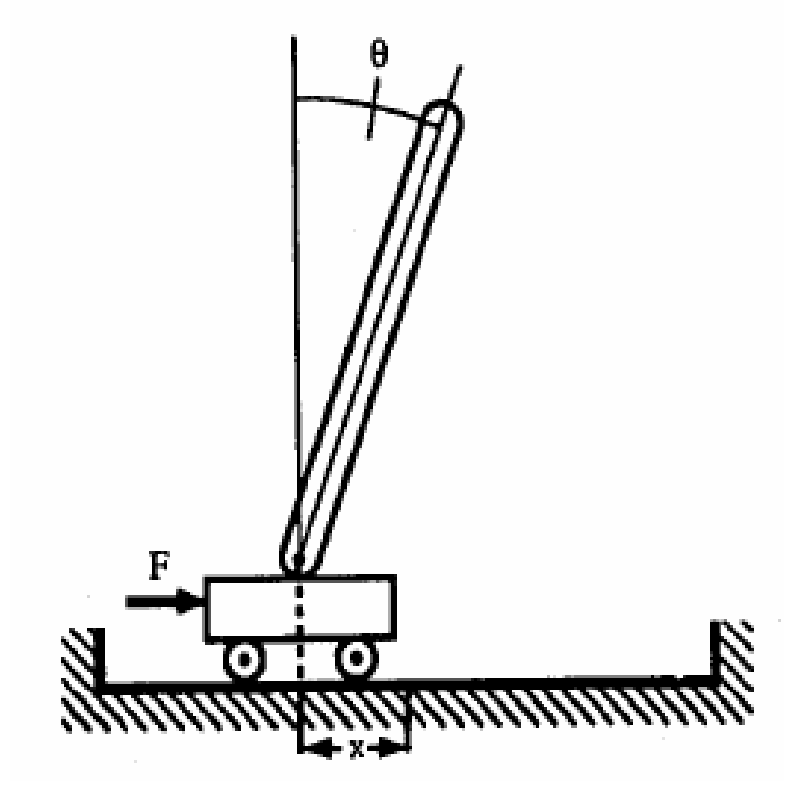
\includegraphics[width=5cm]{cart-pole.png}
\caption{Cart-Pole System\cite{Brownlee2005}}
\label{cart-pole}
\end{center}
\end{figure}

In order to control the system, we should apply a force to the
cart-pole system. Normally the force can not be zero (hence the
bang-bang control). A successful control case is to let the cart
remain in the range of the restriction and the pole doesn't fall down
in the control period.\\

So in this system the input vector is $(x_t, x'_t, \theta_t, \theta '_t, F_t,
\rho)$. And the output vector, ($x_{t+1}, x'_{t+1}, \theta_{t+1},
\theta '_{t+1}$), represents the state of the system after time $\rho$
applying force $F_t$ to state $(x_t, x'_t, \theta_t, \theta '_t$. In
\cite{Brownlee2005}, the equations of accelerates for both position and
angle resulted from the force are given as follow:
\begin{center}
\begin{equation}\label{PH:theta2}
\theta_{t} '' = \frac{g \sin{\theta_t} +
  \cos{\theta_t}[\frac{-F_t-m_p l
    {\theta_t '}^2\sin{\theta_t}}{m_c+m_p}]}{l[\frac{4}{3}-\frac{m_p \cos^2{\theta_t}}{m_c+m_p}]}
\end{equation}
\begin{equation}\label{PH:x2}
x'' = \frac{F_t + m_p l [\theta_t '^2 \sin \theta_t - \theta''_t \cos \theta_t]}{m_c+m_p}
\end{equation}
\end{center}

By using the given equations, we can easily simulate this
system. First we set a small $\rho$ (2ms) deviding the whole time
sequence into small time slices. Then for each time slice, its state
is the output from the input whose state are taken from the previous
time slice.
\begin{center}
\begin{equation}\label{PH:x}
x_{t+1} = x_t + \rho x'_t, x'_{t+1} = x'_t + \rho x''_t
\end{equation}
\begin{equation}\label{PH:theta}
\theta_{t+1} = \theta_t + \rho \theta'_t, \theta'_{t+1} = \theta'_t + \rho \theta''_t
\end{equation}
\end{center}

Additionally, to achieve the bang-bang control, each time slice we
need to decide which force we are given to the cart. In a simple case,
we could just drive the system with forces in the same magnitude (two
directions). For the direction of the forces, we use the following
equation to decide \cite{Brownlee2005}.
\begin{center}
\begin{equation}\label{PH:bangbang}
F_t = F_m sgn (k_1 x_t + k_2 x'_t + k_3 \theta_t + k4 \theta'_t)
\end{equation}
\end{center}

In this equation, $F_m$ is the constant magnitude of the forces and
the sign function decide on which direction the forces should apply
controlled by the parameter $(k_1, k_2, k_3, k_4$. However, when the
system is far away from the stable state, this control function could
fail at last. The figure \ref{fail-control} gives us an example of the
control's failure.\\

\begin{figure}[h!]
\begin{center}
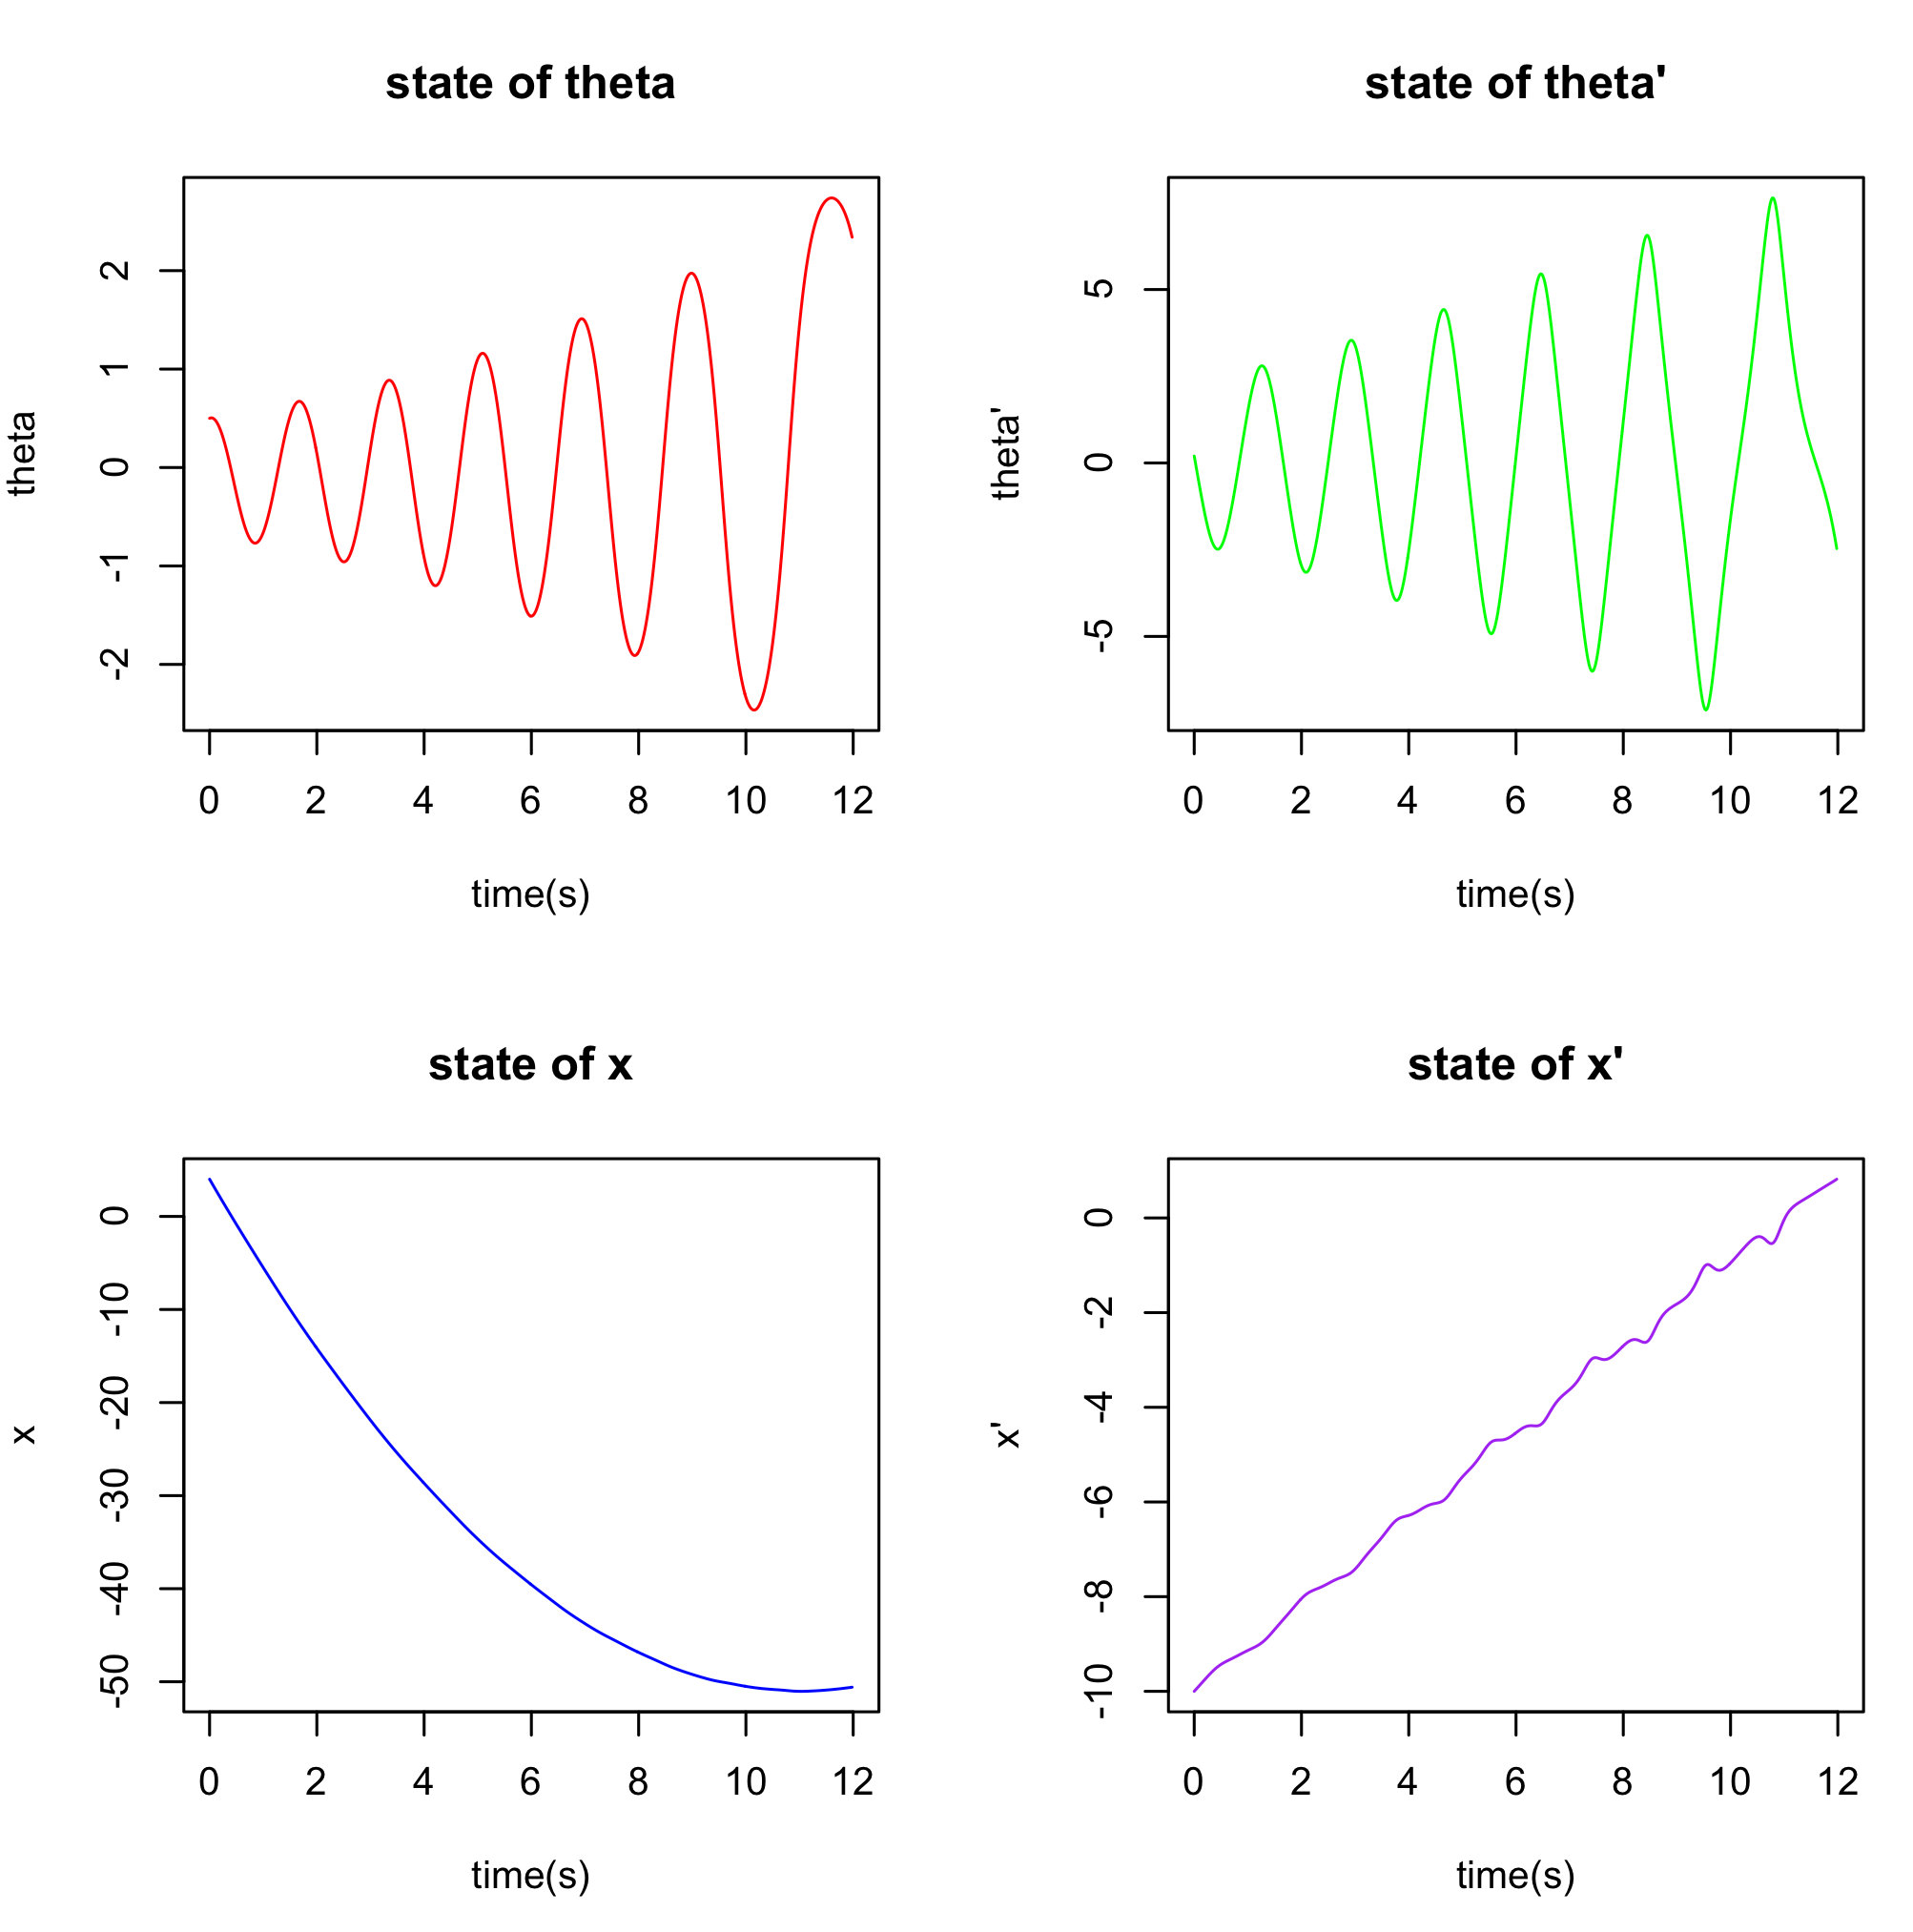
\includegraphics[width=14cm]{fail-control.png}
\caption{An example of failed control}
\label{fail-control}
\end{center}
\end{figure}

In figure \ref{fail-control}, the initial state of the system is too
far away from stable and the forces $F_m$ is too weak, so at last,
$\theta$ (angle of pole) is out of the bound $(-1, 1)$, which indicates
the control is actually failed. When we set the initial state and the
force at a suitable value, the system behavior would be seen like in
figure \ref{success-control}.\\

\begin{figure}[h!]
\begin{center}
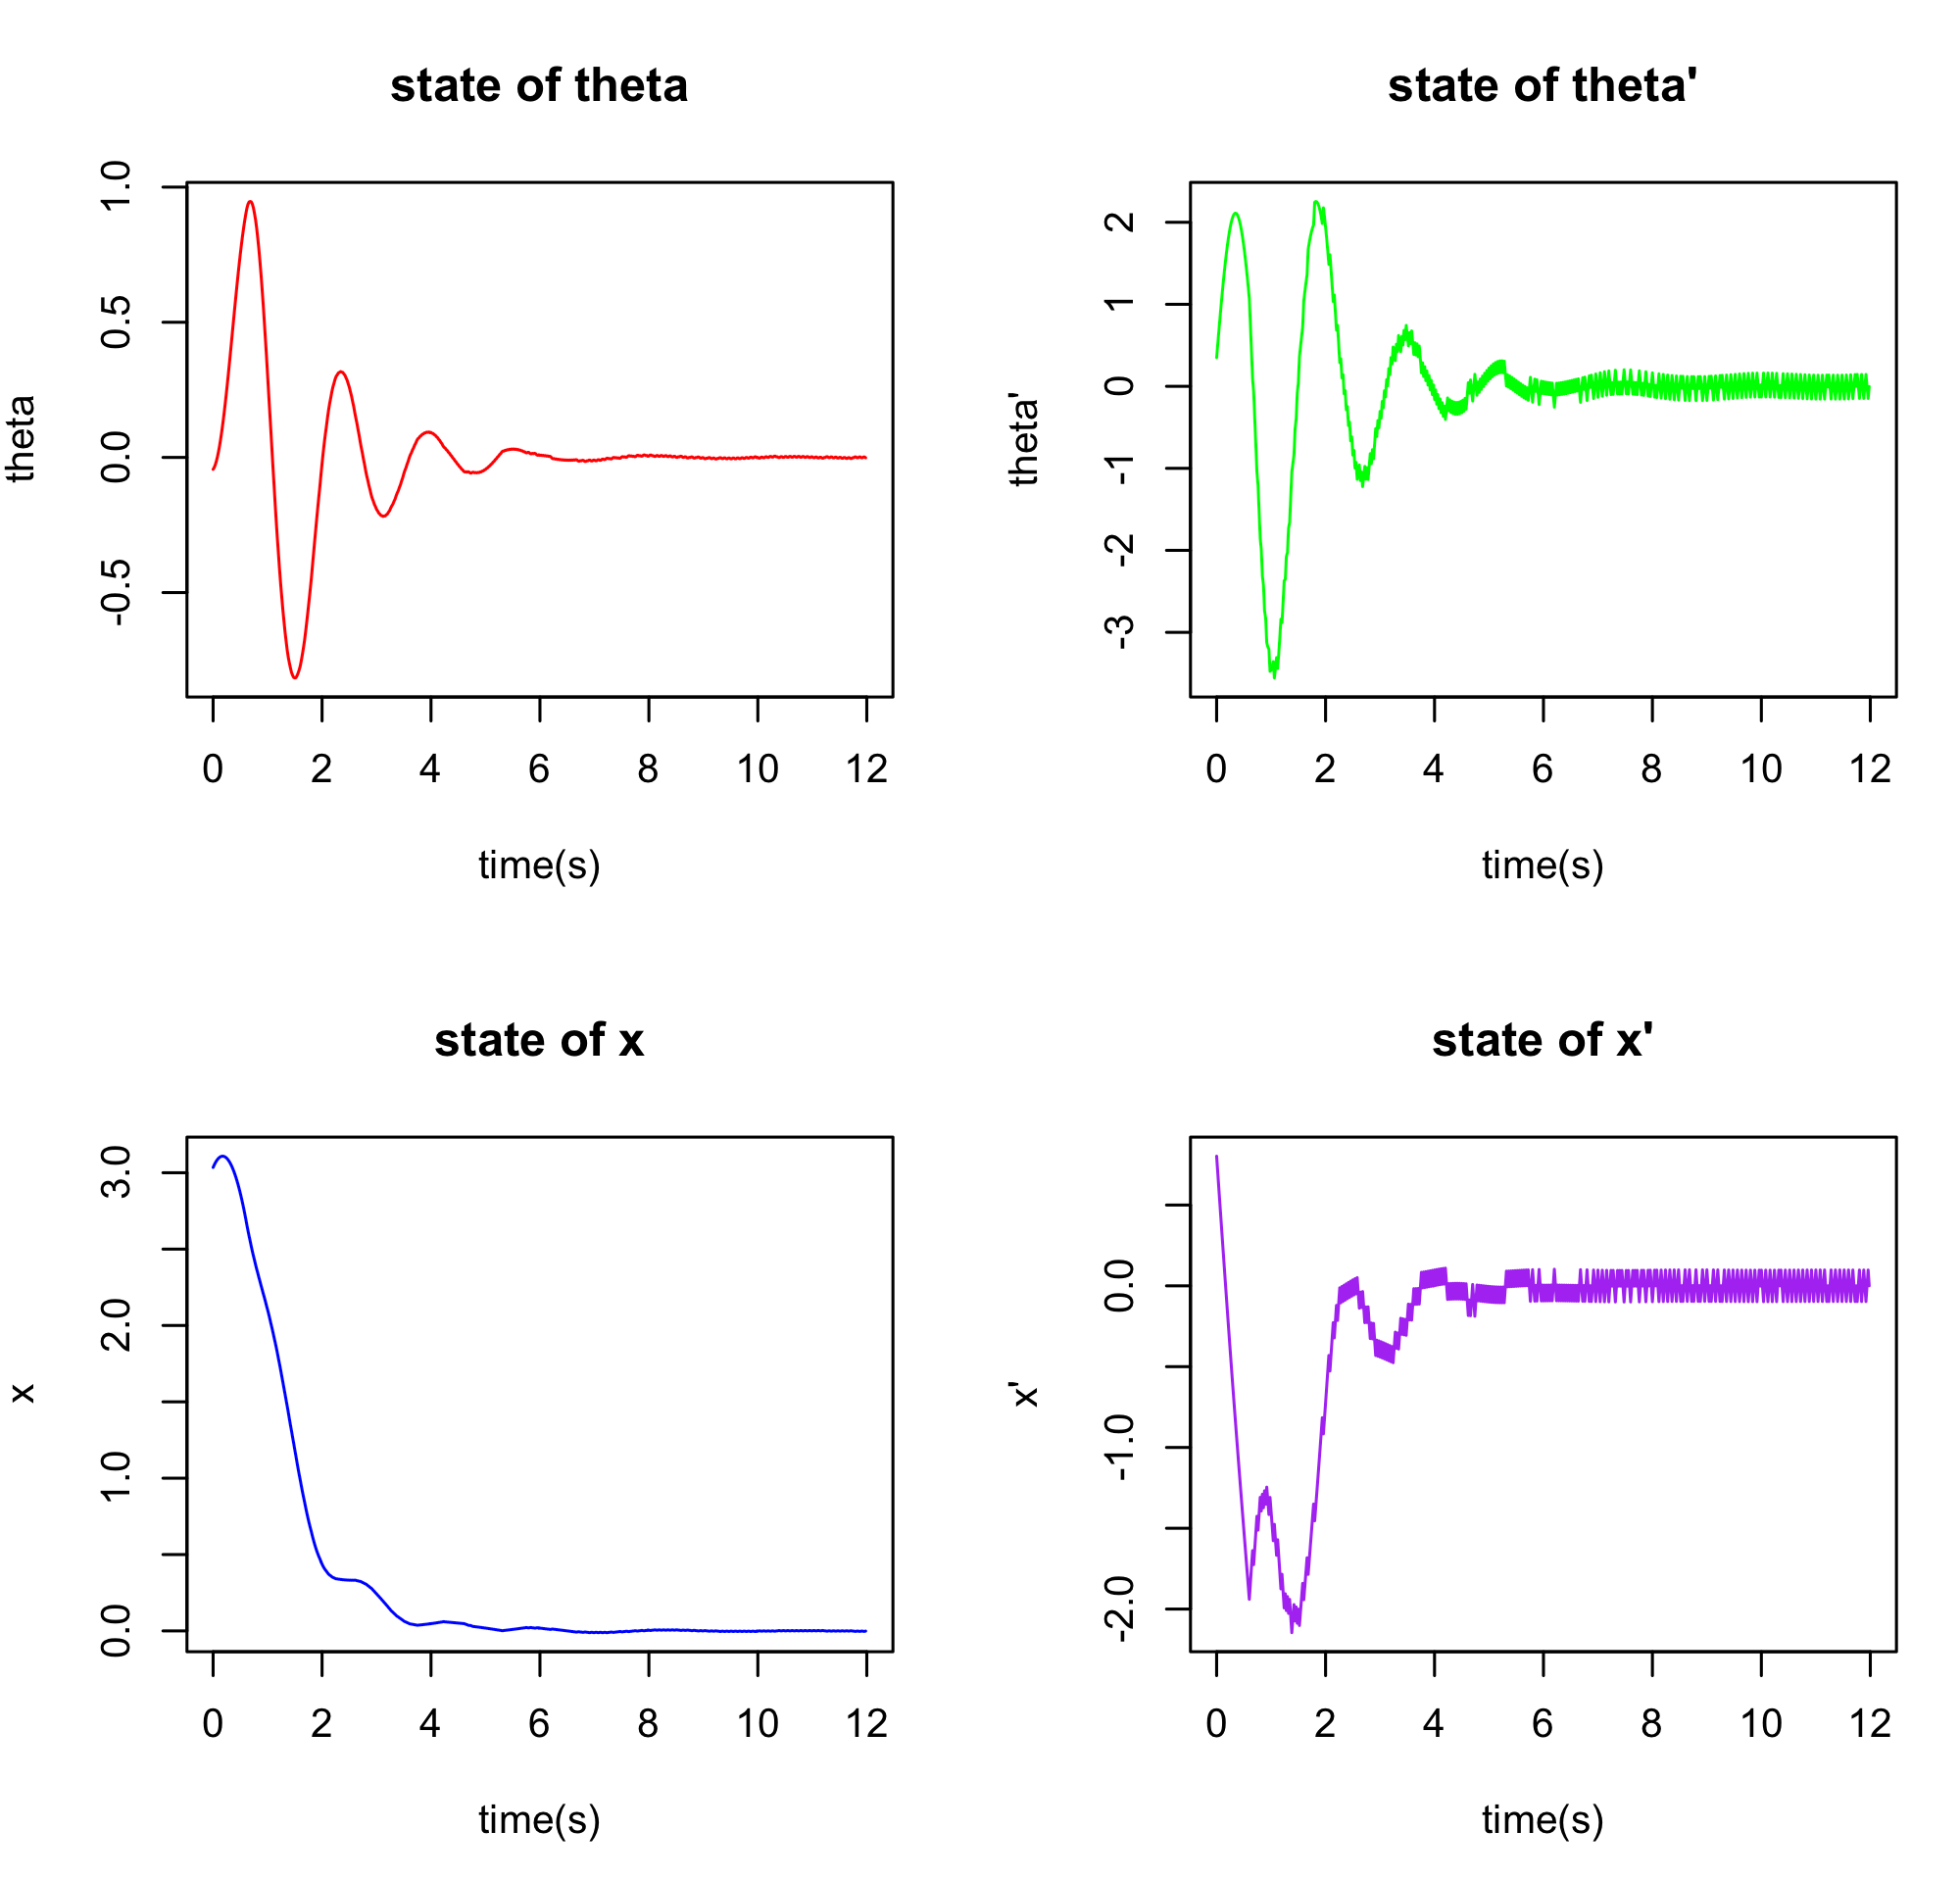
\includegraphics[width=14cm]{success-control.png}
\caption{An example of successful control}
\label{success-control}
\end{center}
\end{figure}

\section{Learning and Controlling the System}
In this section, we will first go through the basics of the gaussian
process. Then applications of Gaussian process will be discussed.
Applications in a dynamic system using gaussian process could be
devided into two part. Applications of the first part are doing the
learning job. They mainly try to predict the behavior of the
system. Mostly, an initial state of the system is given and the
applied forces at each time slice are also provided. Another part
covers the applications trying to control this system. So, in these
application scenes, each time slice, the state can be retrieved. The
application should decide the force with its maginitude and
direction.\\
\subsection{Gaussian Process}
Guassian process is a generalization of the Gaussian probability
distribution. It is defined as follow \cite{Rasmussen2006}:
\begin{mydef}[Gaussian Process]
A Gaussian process is \textit{a collection of random variables, any finite
number of which have a joint Gaussian distribution}.
\end{mydef}

In the above definition, we could find that though Gaussian process is
a definition over an infinite dimensional data, the vector we really
deal with is always a finite one. A Gaussian process is compeletely
sprcified by a mean function and a covariance function. 
\begin{center}
\begin{equation}
f(x) \sim GP(m(x), k(x, x))
\end{equation}
\begin{equation}
m(x) = E[f(x)], k(x, x') = E[(f(x)-m(x))(f(x')-m(x'))]
\end{equation}
\end{center}
Normally, for simplicity, we take the mean function as zero and the
most common used covariance function is the \textit{squarred
  exponential} covariance function.
\begin{center}
\begin{equation}
m(x) = 0, k(x, x') = e^{-\frac{1}{2}|x-x'|^2}
\end{equation}
\end{center}
In the regression problem, we have some sampled observations, denoted
as training input set $X$. Its observed training output (with noise) would be $\textbf{y}$. On the other
way, $X^*$ is the test input and we want to get the test output
$f^*(x)$. So in this case, the joint distribution over the
$(\textbf{y}, f^*(x))$ according to the prior is,
\begin{center}
\begin{equation}
\begin{bmatrix}
\textbf{y} \\
f^*(x)
\end{bmatrix} \sim N (0,
\begin{bmatrix}
K(X, X) + \sigma^2\textbf{I} & K(X, X^*) \\
K(X^*, X) & K(X^*, X^*)
\end{bmatrix} )
\end{equation}
\end{center}
To get the posterior distribution over the function $f^*(x)$, the
problem is deriving conditional distribution over the observations. So
here is the \textbf{key predictive equations} of the Gaussian process
regression.
\begin{center}
\begin{equation} \label{GP:Mean}
\bar{f^*} = K(X^*, X)[K(X, X) + \sigma^2\textbf{I}]^{-1}\textbf{y}
\end{equation}
\begin{equation} \label{GP:Cov}
cov{f^*} = K(X^*, X^*) - K(X^*, X)[K(X, X) +
\sigma^2\textbf{I}]^{-1}K(X, X^*)
\end{equation}
\end{center}
So far, the basics of Gaussian process have been covered. In this
project, we mainly use the equations \ref{GP:Mean} and \ref{GP:Cov} to
compute as the core of our Models.

\subsection{The Learning Model}
Learning the behavior of the cart-pole system is based on the
training data that is observed from some pre-runs of the system. At
first, we let this system run a few times with different
set-ups and observe. In this way, we can get the training data which
will be considered as the prior knowledge of our model.\\ 

In our learning model, state of each time slice will be alternatively
predicted based on the previous time slice. And in the cart-pole
system, input vectors are 6-dimensional and outputs are 4-dimensional
vectors. So at each time slice, we solve each element in
the output vector seperately and put them all together with as the
output of whole one-step prediction process. Figure
\ref{learning-model} shows the structure of the learning model.\\

\begin{figure}[h!]
\begin{center}
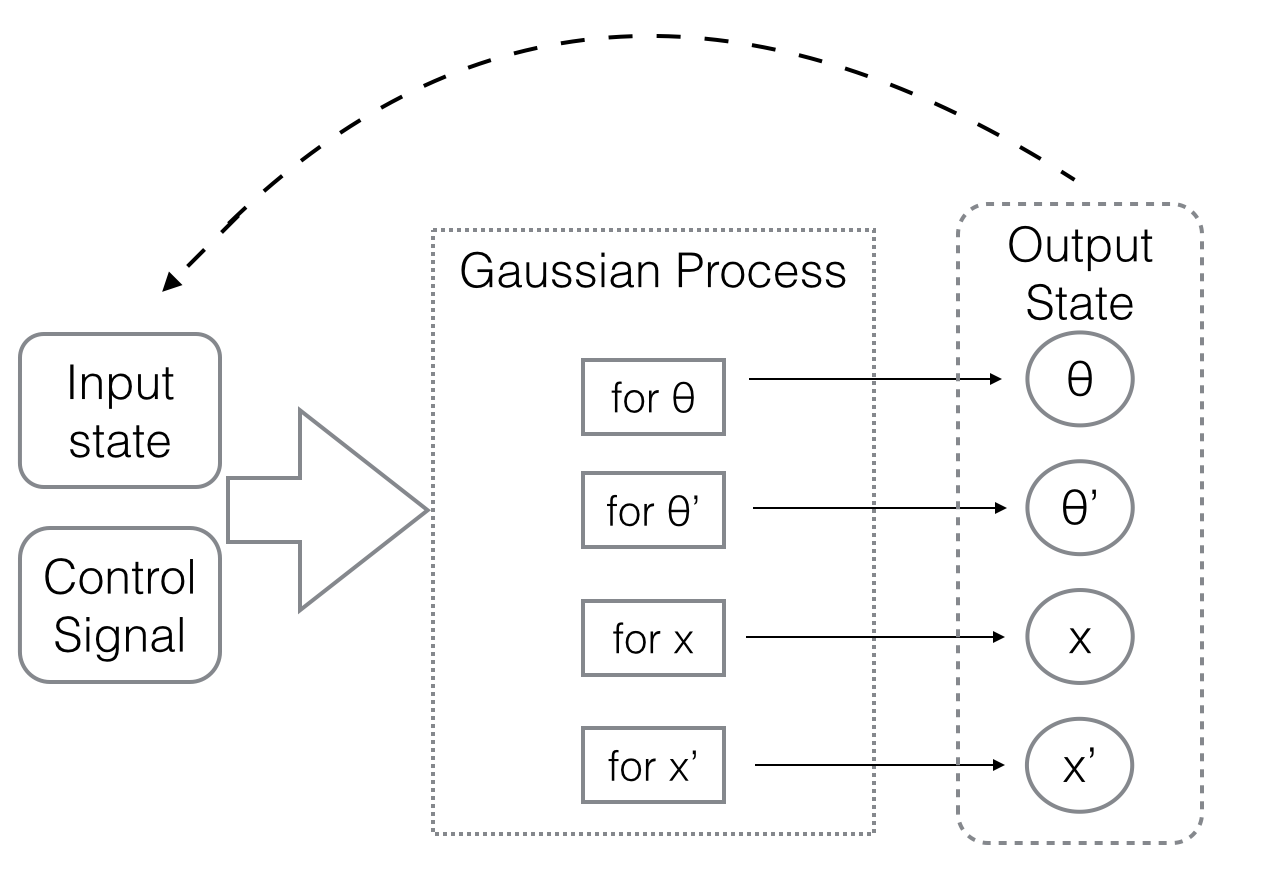
\includegraphics[width=8cm]{learning-model.png}
\caption{Design of Learning Model}
\label{learning-model}
\end{center}
\end{figure}

\subsection{The Control Model}
In the control scene, the input of the model at each time slice $t$ is the
state of the cart-pole system. In response to the state, our model
need to output the magnitude and direction of the force applying to
the system. So here, we denote the input as $s_t$. And the
output is $F_t$.\\
\begin{figure}[h!]
\begin{center}
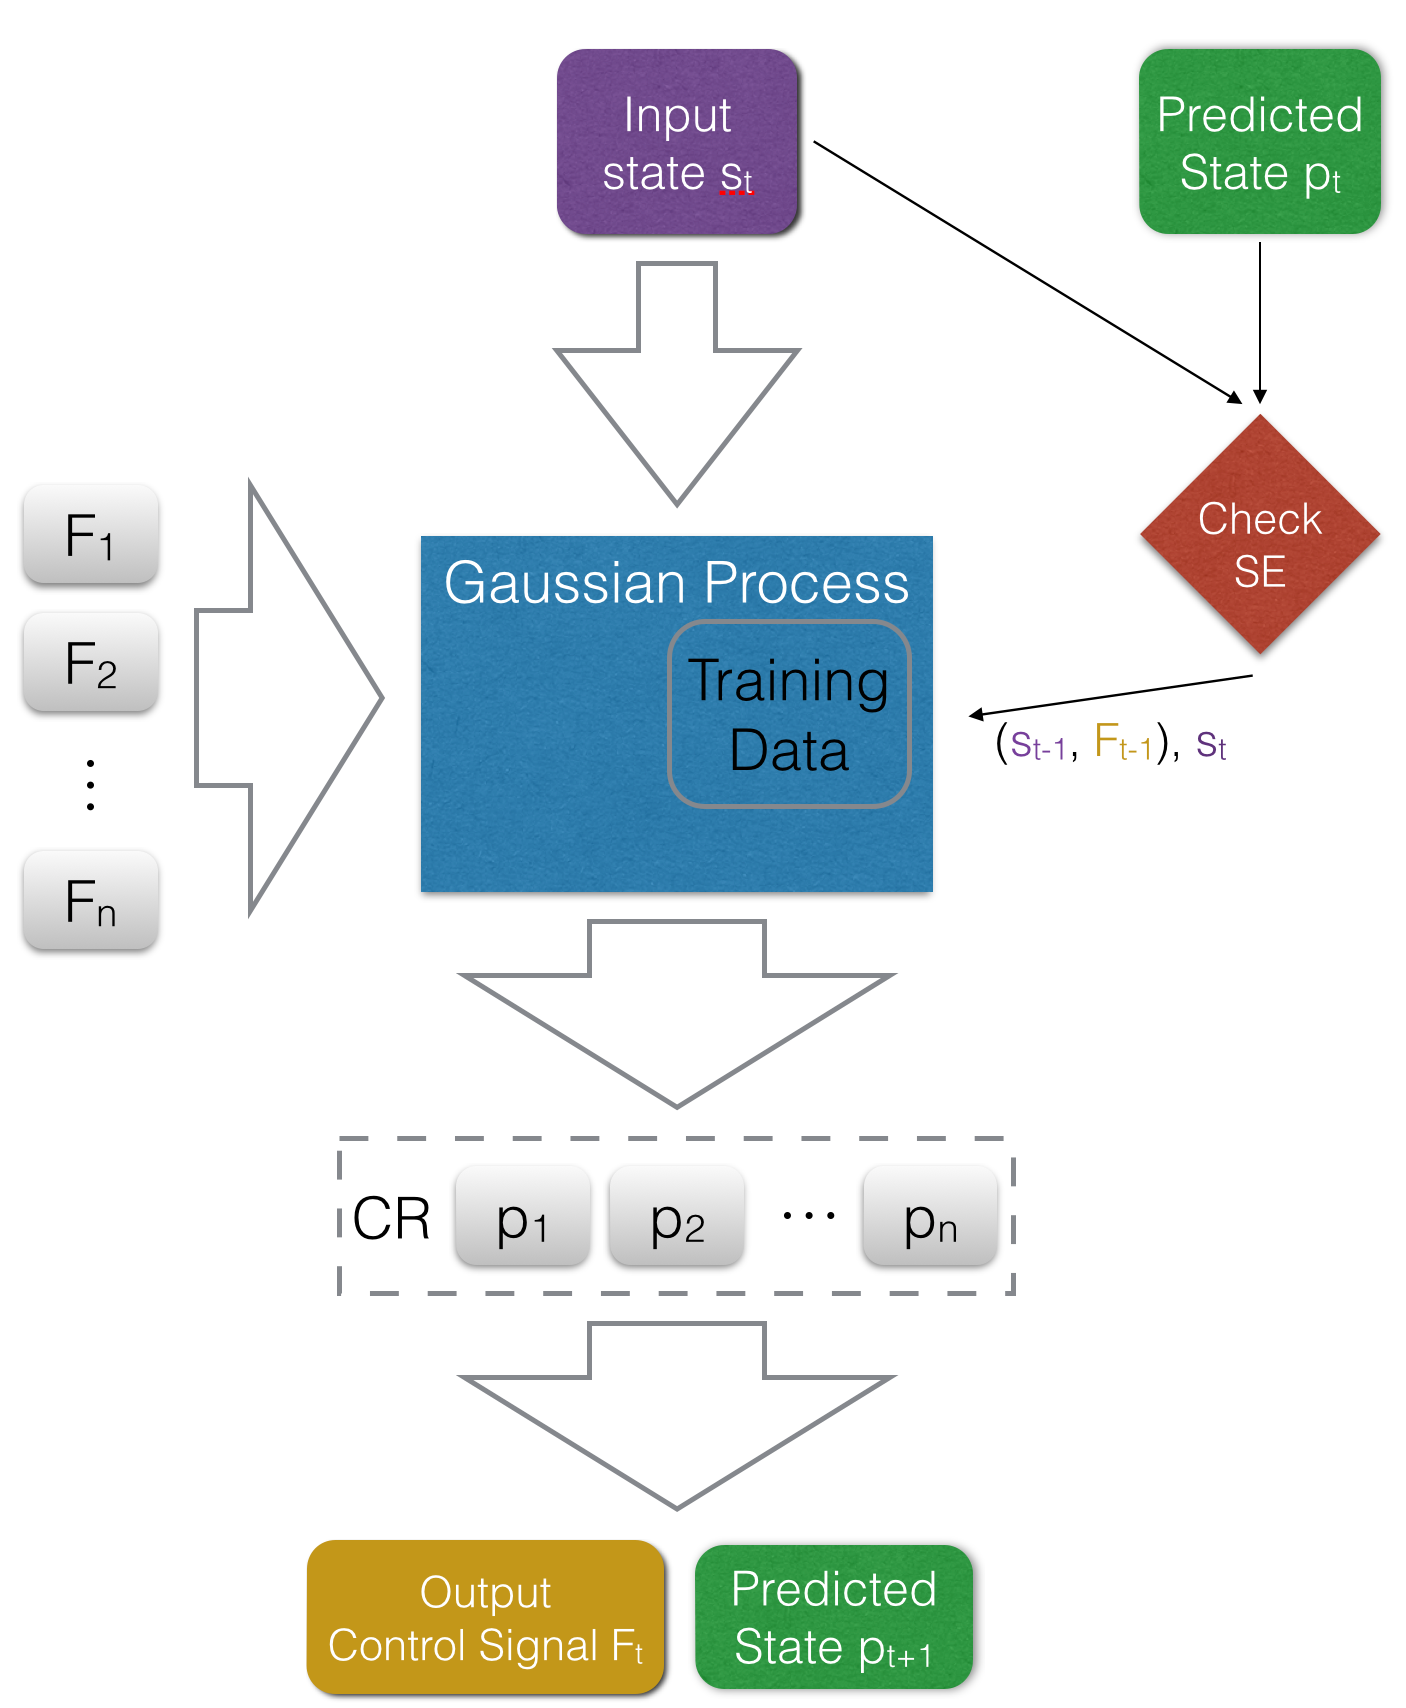
\includegraphics[width=8cm]{control-model.png}
\caption{Design of Control Model}
\label{control-model}
\end{center}
\end{figure}

In order to determine $F_t$ as the output control signal. We
use Gaussian process to predict the states after applying several
possibilities of forces (for each force $F_i$ applying to the system,
the prediction we denoted as $p_i$). Among these predictions, we could
choose the best one based on a criteria function $CR$.
\begin{center}
\begin{equation}
F_t = argmin_i{CR(p_i)}
\end{equation}
\begin{equation} \label{criteria}
CR(p_i) = t_1 |p_i.x'| + t_2 |p_i.\theta| + t_3 |p_i.\theta'|
\end{equation}
\end{center}

In the equation \ref{criteria}, $t_1, t_2, t_3$ are parameters that
specify the property of the choosing criteria. The larger $t_i$ is,
the more import its element would be considered. For example, when the
pole fall down, the system could never get back to the valid state
again. So the angel of the pole $\theta$ could be considered as the most
essiential element and we can set $t_2$ to be much larger than others.\\

Another issue that should be considered is that our control model
initially can give nearly no training data to the Gaussian process. So
it should learn from the controlling process of the cart-pole
system. Hence each time slice, when our model gets the input
$s_t$, it could consider the state of the previous slice
and the control sign applied $(s_{t-1}, F_{t-1})$ as
a function input. And the pair 
$((s_{t-1}, F_{t-1}), s_t)$
can be used as a pair of training data.
\begin{center}
\begin{equation}
s_t = f(s_{t-1}, F_{t-1})
\end{equation}
\end{center}

However, in fact, the gaussian process model should not take all pairs
as the training data. As when the data size increases, the process
time would increase dramatically due to the complexity of the Gaussian
process. So, the control model should also decide
which data it should learn or not.
 
In out model, the prediction from gaussian process and the real
observation will be compared (using sum of squared error). If the sum
of squarred error is below a certain level (for example, 0.001), the
model can ignore this data. Otherwise the model should add this data
to the training data, and continue to learn using the new training data. The whole process of the model could be
found in figure \ref{control-model}.\\

\section{Implementation Details}
In this project, we basically run our Gaussian process based models on
the cart-pole system. The paramters which are used in the system and
model are show in table \ref{tab:parameters}, the setting of these
parameters could be find in the file \textbf{'CommonVar.R'}.\\

\begin{table}
\centering
\begin{tabular}{c|c}
\hline
l & 0.5  \\ \hline
$M_p$ & 0.1 \\ \hline
$M_c$ & 1  \\ \hline
$k_1$ & -1  \\ \hline
$k_2$ & -1  \\ \hline
$k_3$ & 1  \\ \hline
$k_4$ & -0.1  \\ \hline
$\rho$ & 0.02  \\ \hline
\end{tabular}
\caption{Table of Parameters}
\label{tab:parameters}
\end{table}

First, we implement two processing core. One is the simulation of a
real physical system. The implementation of this core is based on the
equations (\ref{PH:theta2}) and (\ref{PH:x2}). By using (\ref{PH:x})
and (\ref{PH:theta}), we could simulate the whole behavior of the
system as a real physical system. Detailed implementation could be
found in the file \textbf{'PhysicalCore.R'}.\\

Another processing core is based on Gaussian process, it will take a
state and force as input, and give a prediction on the state of the
system after time $\rho$. The core's implementation could be found in
the file \textbf{'GaussianProcessRegression.R'}. As a query of state
will use the Gaussian process 4 times (each element in the output
vector once), so in order to get the next state, function
\textit{gpNextState} in the file \textbf{'GuassianProcessCore.R'}
will be useful.\\

The running of Gaussian process needs training data. This is especially
important in the learning model. The training data is obtained first
by setting the initial state and the magnitude of force $F_m$ in
equation (\ref{PH:bangbang}). Then the system is simulated using a
physical core and controlled by the method in equation
(\ref{PH:bangbang}). The training data is thus retrieved from the
state-to-state transformation between all time slices. The training
data generation can be found in the file
\textbf{'DataGeneration.R'}, it will save the training data in the
file \textit{'ModelData.RData'}.\\

After the generation of training data, we could stimulate the system
behavior using GaussianProcess. Our learning model simulates the
system using the same control method as in the data generation
process. Implementation of the simulation using Gaussian process can
be found in the file \textbf{'DataSimulation.R'}, it will read the
data from \textit{'ModelData.RData'} and save its learning results to
\textit{'GP\_Results.RData'}. The same time of simulation of the
system using Gaussian process, we are simulate the system using the
physical model at the same time in order to compare. Simulation
results will be stored in file \textit{'Sim\_Results.RData'}\\

As for the control model, we choose forces from -5 to 5 (intergers) at
each step to use as the control signal. At each step, the prediction states
from different forces will be compared and choosed based on the
equation \ref{criteria}. The parameters in (\ref{criteria}) will all be
set to 1 in our case. As for decision on learning, we check the sum of
squared error. If sum of squared error between states predicted by
Gaussian process and real observation is larger than 0.001, we will
learn the data. The implementation of this model is in the file
\textbf{'ControlSimulation.R'}. The result will be stored in the file \textit{'Sim\_Results.RData'}.\\

\section{Result Analysis}
\subsection{Learning using Gaussian Process}
In the learning model, we need to choose the trainning data for the
gaussian process. Here, we set the same initial state for the system
(see table \ref{tab:initial}).
\begin{table}
\centering
\begin{tabular}{c|c}
\hline
$\theta_{initial}$ & -0.15 \\ \hline
$\theta'_{initial}$ & -1 \\ \hline
$x_{initial}$ & 2 \\ \hline
$x'_{initial}$ & 3 \\ \hline
\end{tabular}
\caption{Unified Initial State of the Learning Process}
\label{tab:initial}
\end{table}
We then set $F_m$ to different values, and let the system run several
times starting from the initial state we given. Figure
\ref{learning-result1} shows the learning results. The training data
for the test in figure \ref{learning-result1} consists of 4 runs
($F_m$ is set from 2N to 5N for each). Each run of the system lasts
for 4 second which, in the physical model, it iterates for 200
times. Among the figures, the {\color{red}red line} is the learning
result from the Gaussian process and the {\color{light-gray} gray lines}
describe the confidential interval of the Gaussian process. The
{\color{green}green line} is the simulation result from the real
physical model. As for the {\color{blue} blue line}, it shows the
result which is from the physical model but takes the states at each
time slice in Gaussian process model's learning result as input.\\
\begin{figure}[!]
\centering
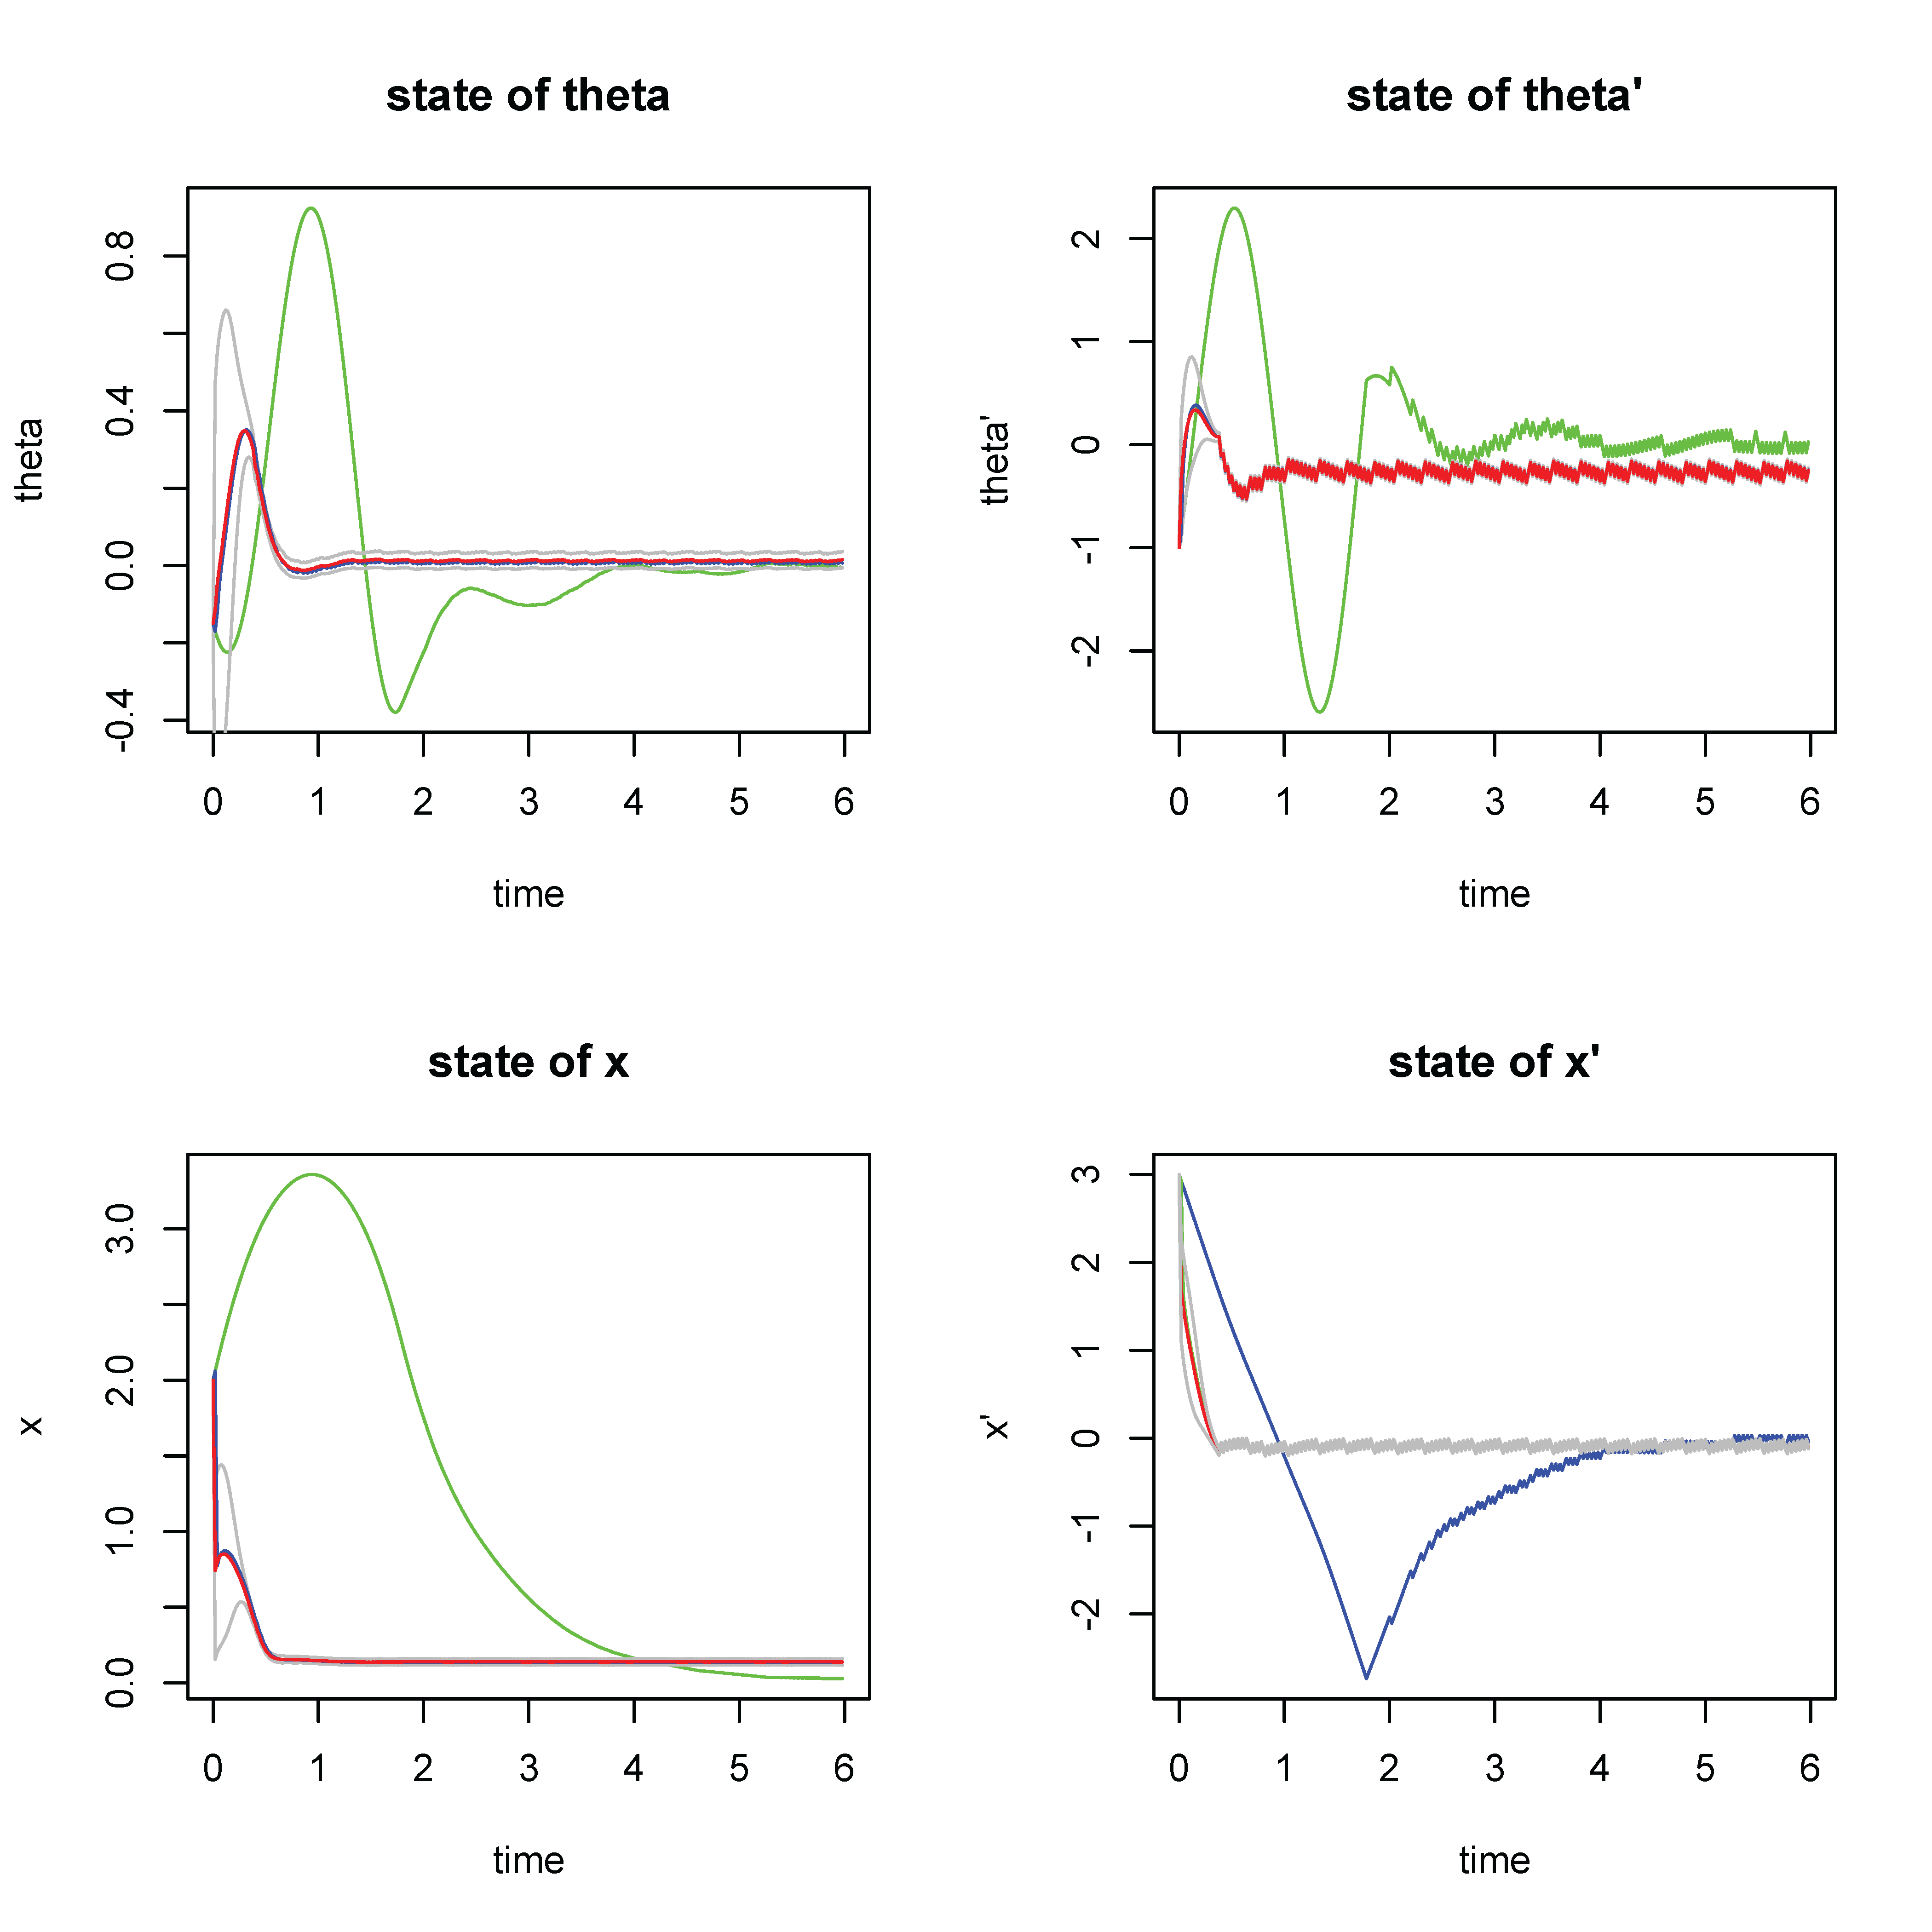
\includegraphics[width=14cm]{learning-result1.png}
\caption{Result of the Learning Dynamic Model, the training data
  consist of runnings using $F_m$ from 2 to 5 (integers) and for each
  running the system runs for 4s (200 steps as $\rho = 0.02s$). The
  test is under $F_m = 3.5N$ and runs for 6s.}
\label{learning-result1}
\end{figure}

As in figure \ref{learning-result1}, the size of training data is
800. We can find that, though the learning result from Gaussian
process ({\color{red}red line}) and the result from the physical model
({\color{green}green line}) are not very identical, the learning
result from Gaussian process ({\color{red}red line}) and the result
from the physical model at each step ({\color{blue} blue line}) are
really closed.\\

We then increase our training data size. We choose $F_m$ from 1 to 10
and let the system runs 4s for each $F_m$. The result is showed in
figure \ref{learning-result2}. As we can see that {\color{red}learning result} from
Gaussian process and the {\color{green}result} from the physical model
are much more close compare to the result showed in figure \ref{learning-result1}.\\

\begin{figure}[!]
\centering
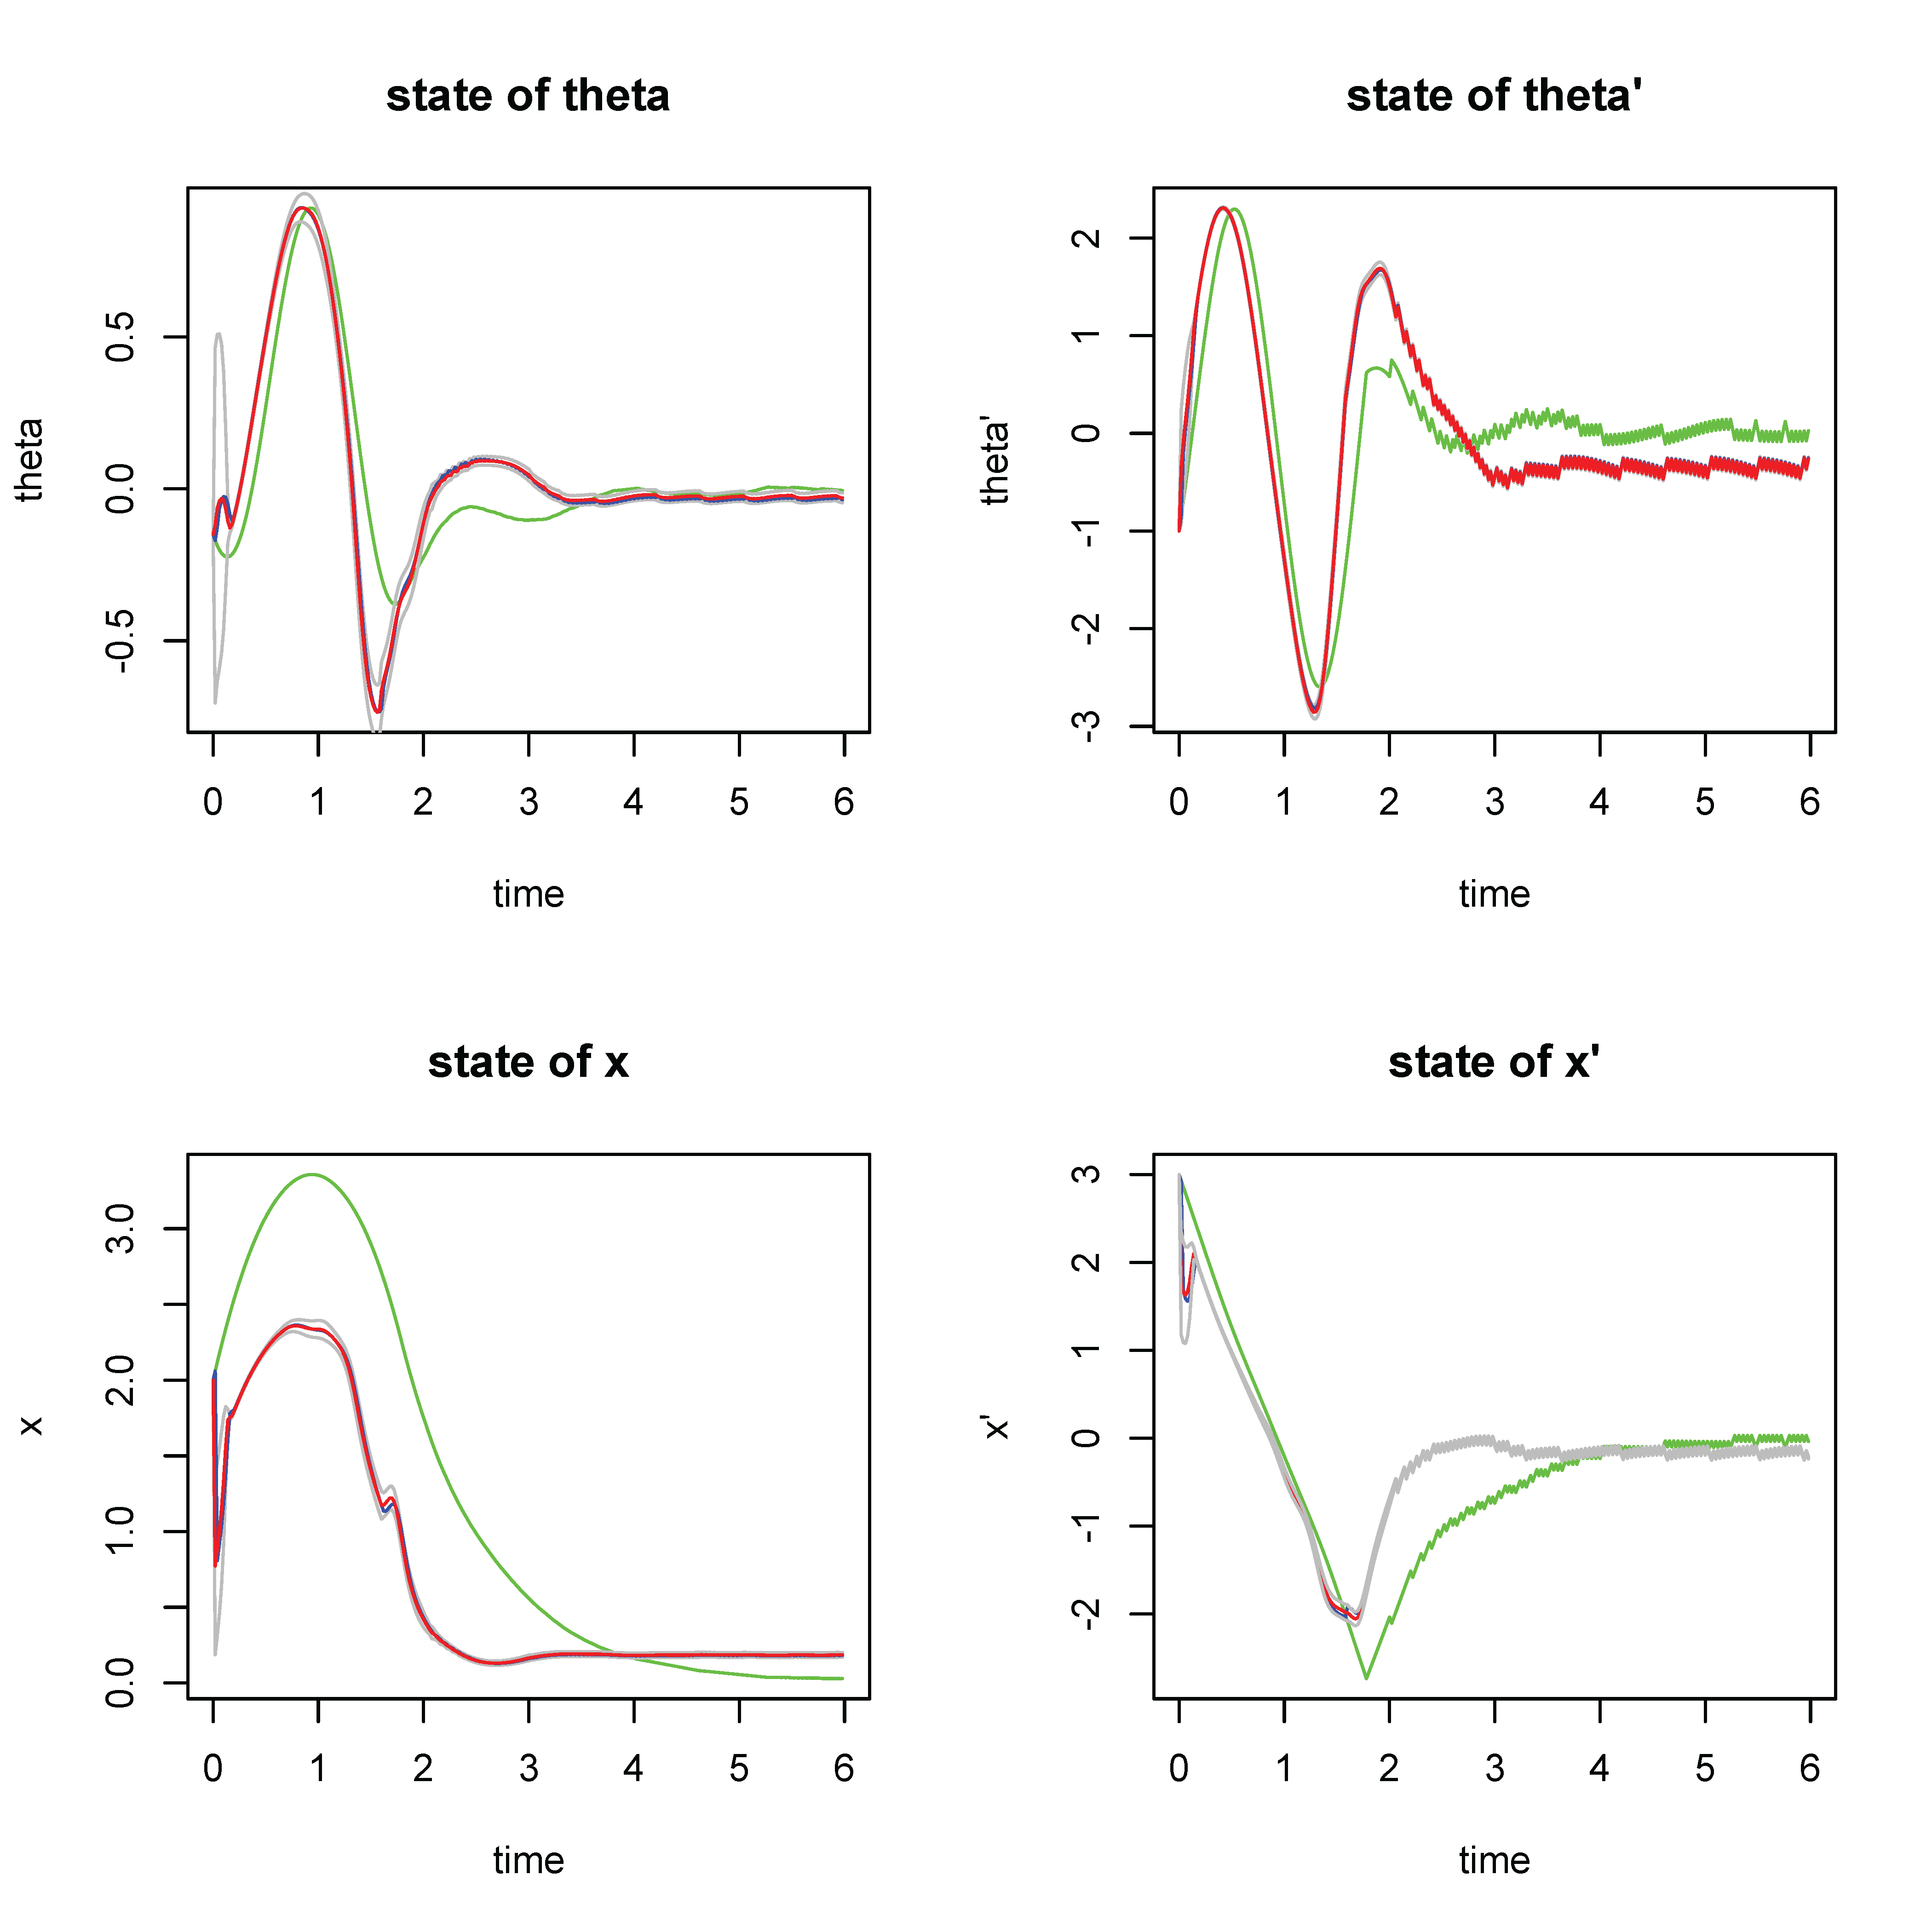
\includegraphics[width=14cm]{learning-result2.png}
\caption{Result of the Learning Dynamic Model, the training data
  consist of runnings using $F_m$ from 1 to 10 (integers) and for each
  running the system runs for 4s (200 steps as $\rho = 0.02s$). The
  test is under $F_m = 3.5N$ and runs for 6s.}
\label{learning-result2}
\end{figure}

So far, we find that, increasing the size of the training data is
really helpful for the Gaussian process. If we want to test the
function value at $\textbf{X}$ but there isn't any observation near
$\textbf{X}$, the predicted value from the Gaussian process should be
more inaccurate. So, as we can see, the learning result of $\theta$ is
much better than the result of $x$. The reason behind this is that
$\theta$ lies in a much more small range than $x$ does. When we let
the system run and learn from the observations, we can say the
observations 'contain' more knowledge of $\theta$ than of $x$.\\

Now, we further increase our size of training data for Gaussian
process. We let the system run under $F_m$ choosing from 1 to 9 and
observe its behavior for 6s. The learning result could be found in
figure \ref{learning-result3}. Now the result from Gaussian process is
nearly identical to the result from the physical simulation.\\

\begin{figure}[!]
\centering
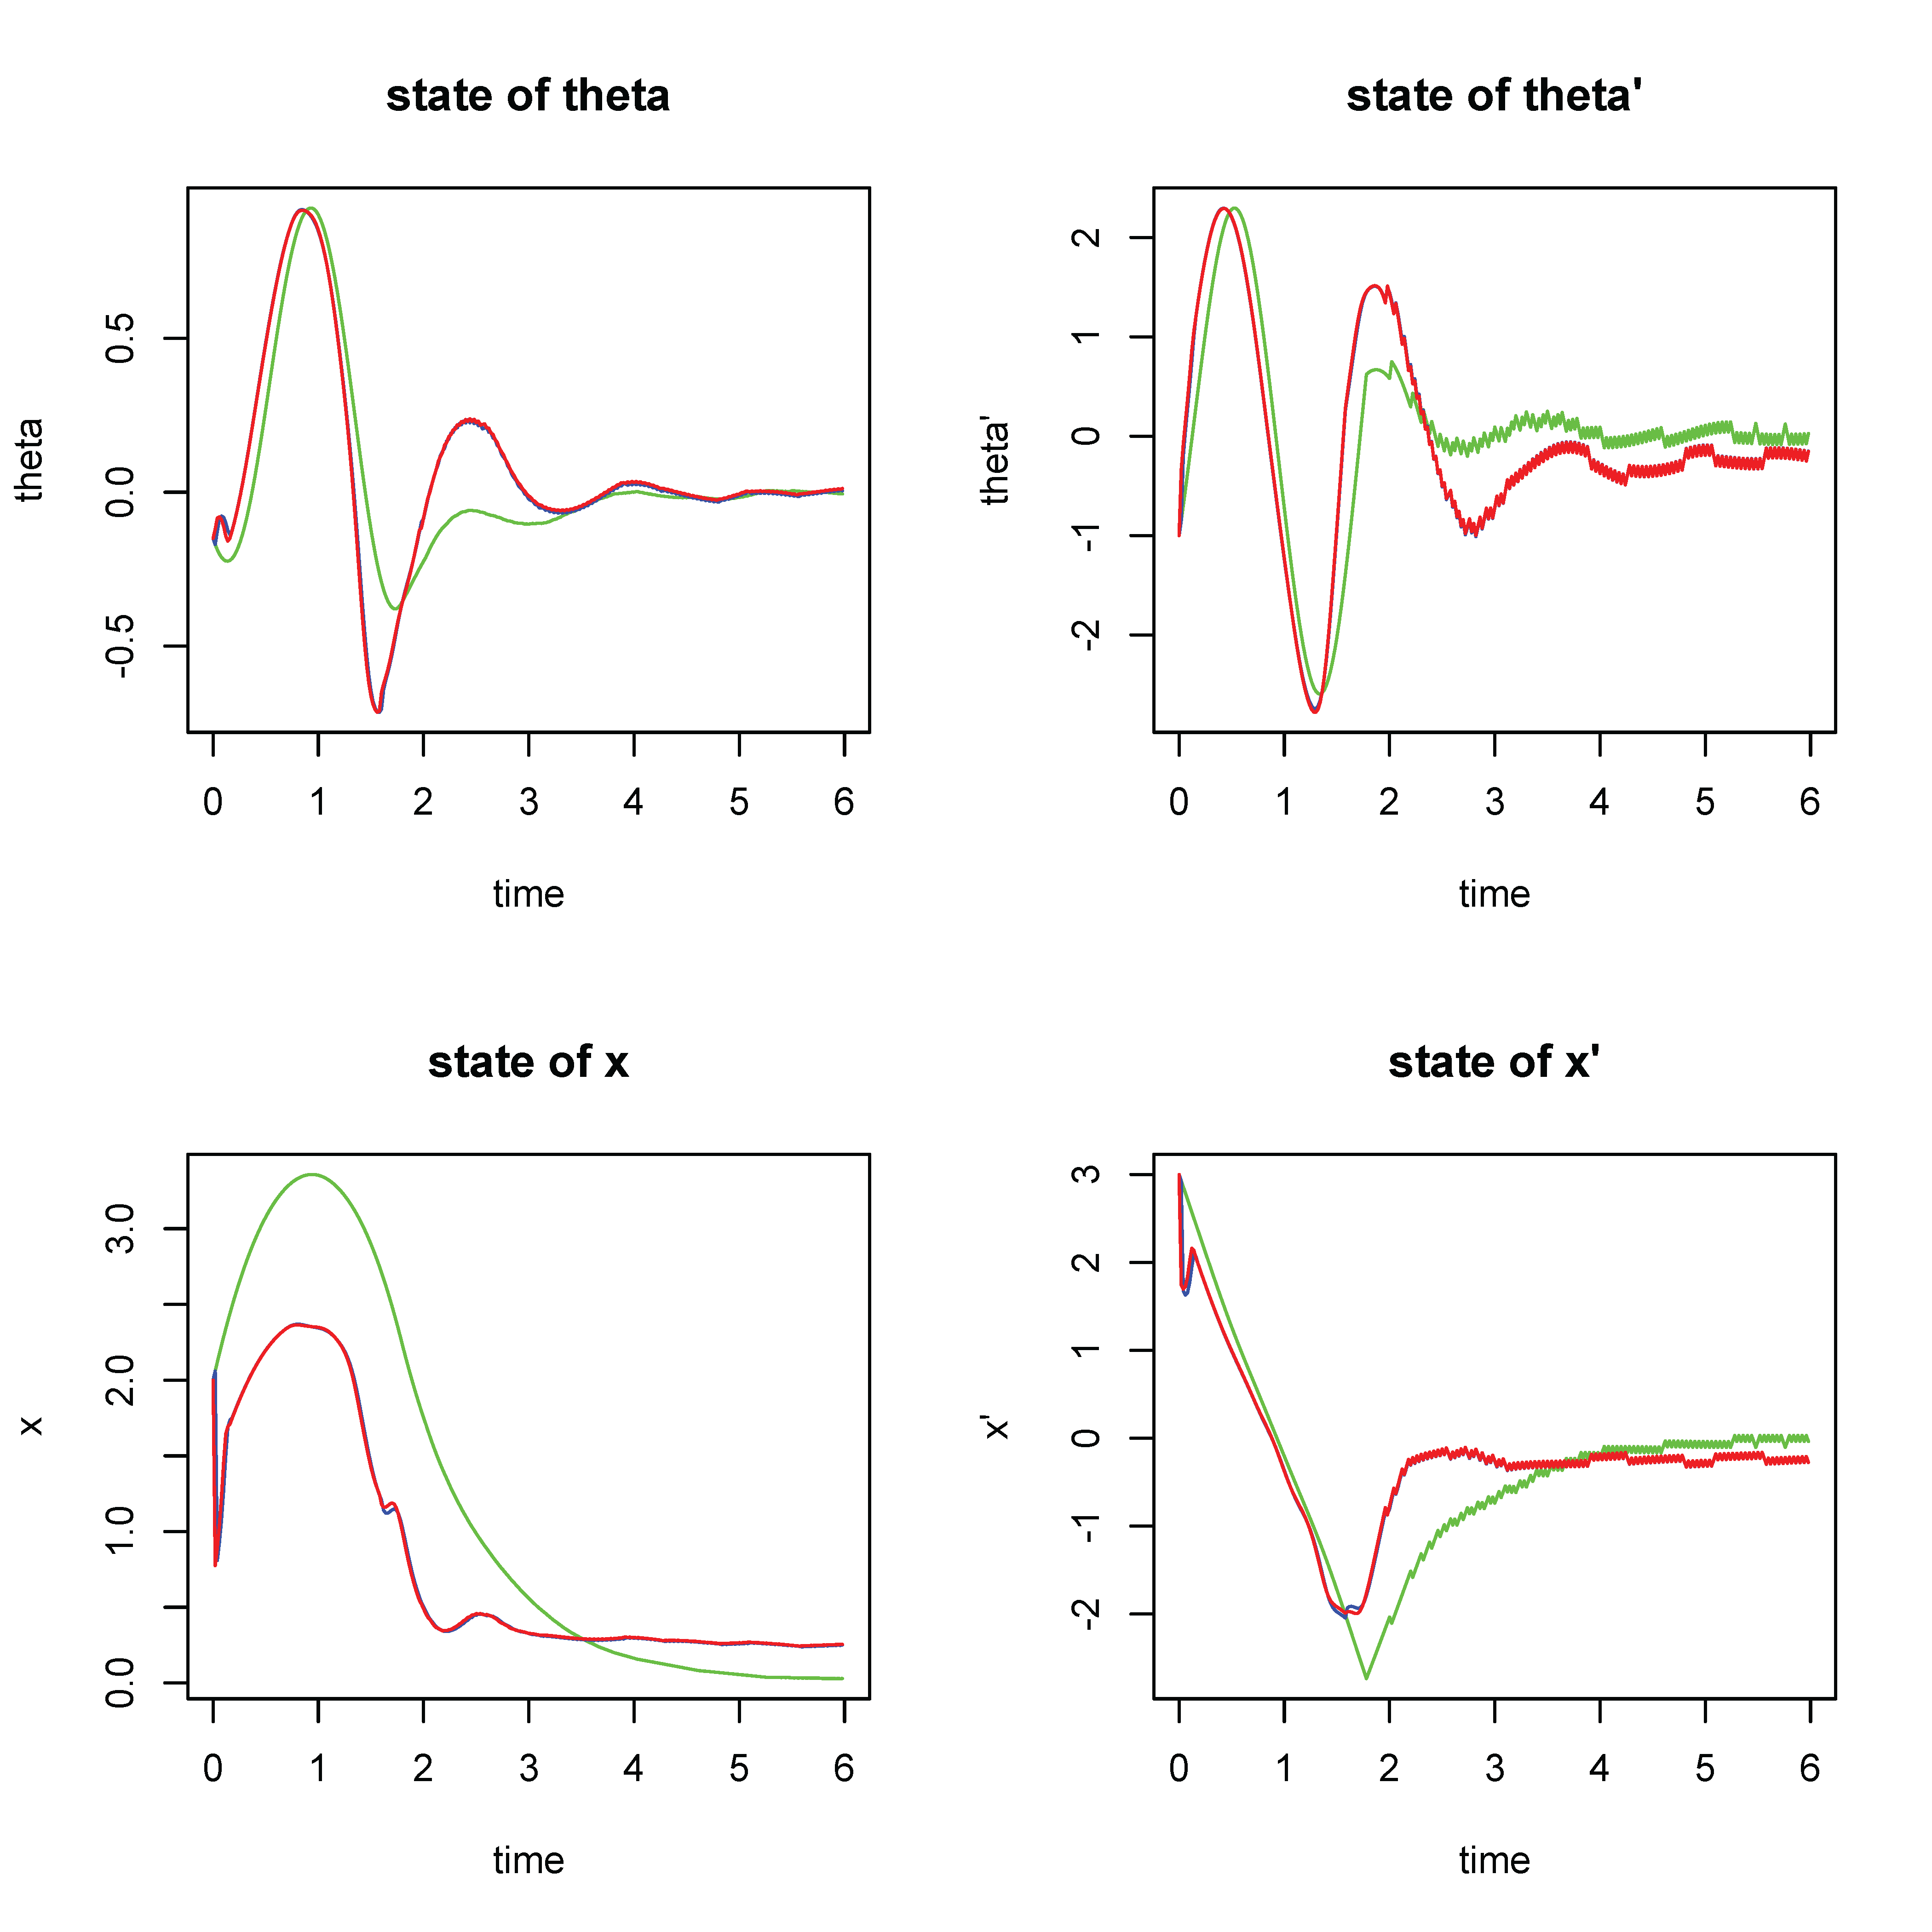
\includegraphics[width=14cm]{learning-result3.png}
\caption{Result of the Learning Dynamic Model, the training data
  consist of runnings using $F_m$ from 1 to 9 (integers) and for each
  running the system runs for 6s (300 steps as $\rho = 0.02s$). The
  test is under $F_m = 3.5N$ and runs for 6s.}
\label{learning-result3}
\end{figure}


\subsection{Controlling using Gaussian Process}

As specified in the previous section, we use our control model to
control a cart-pole system and get the result show in figure \ref{control-result}.\\

\begin{figure}[!]
\centering
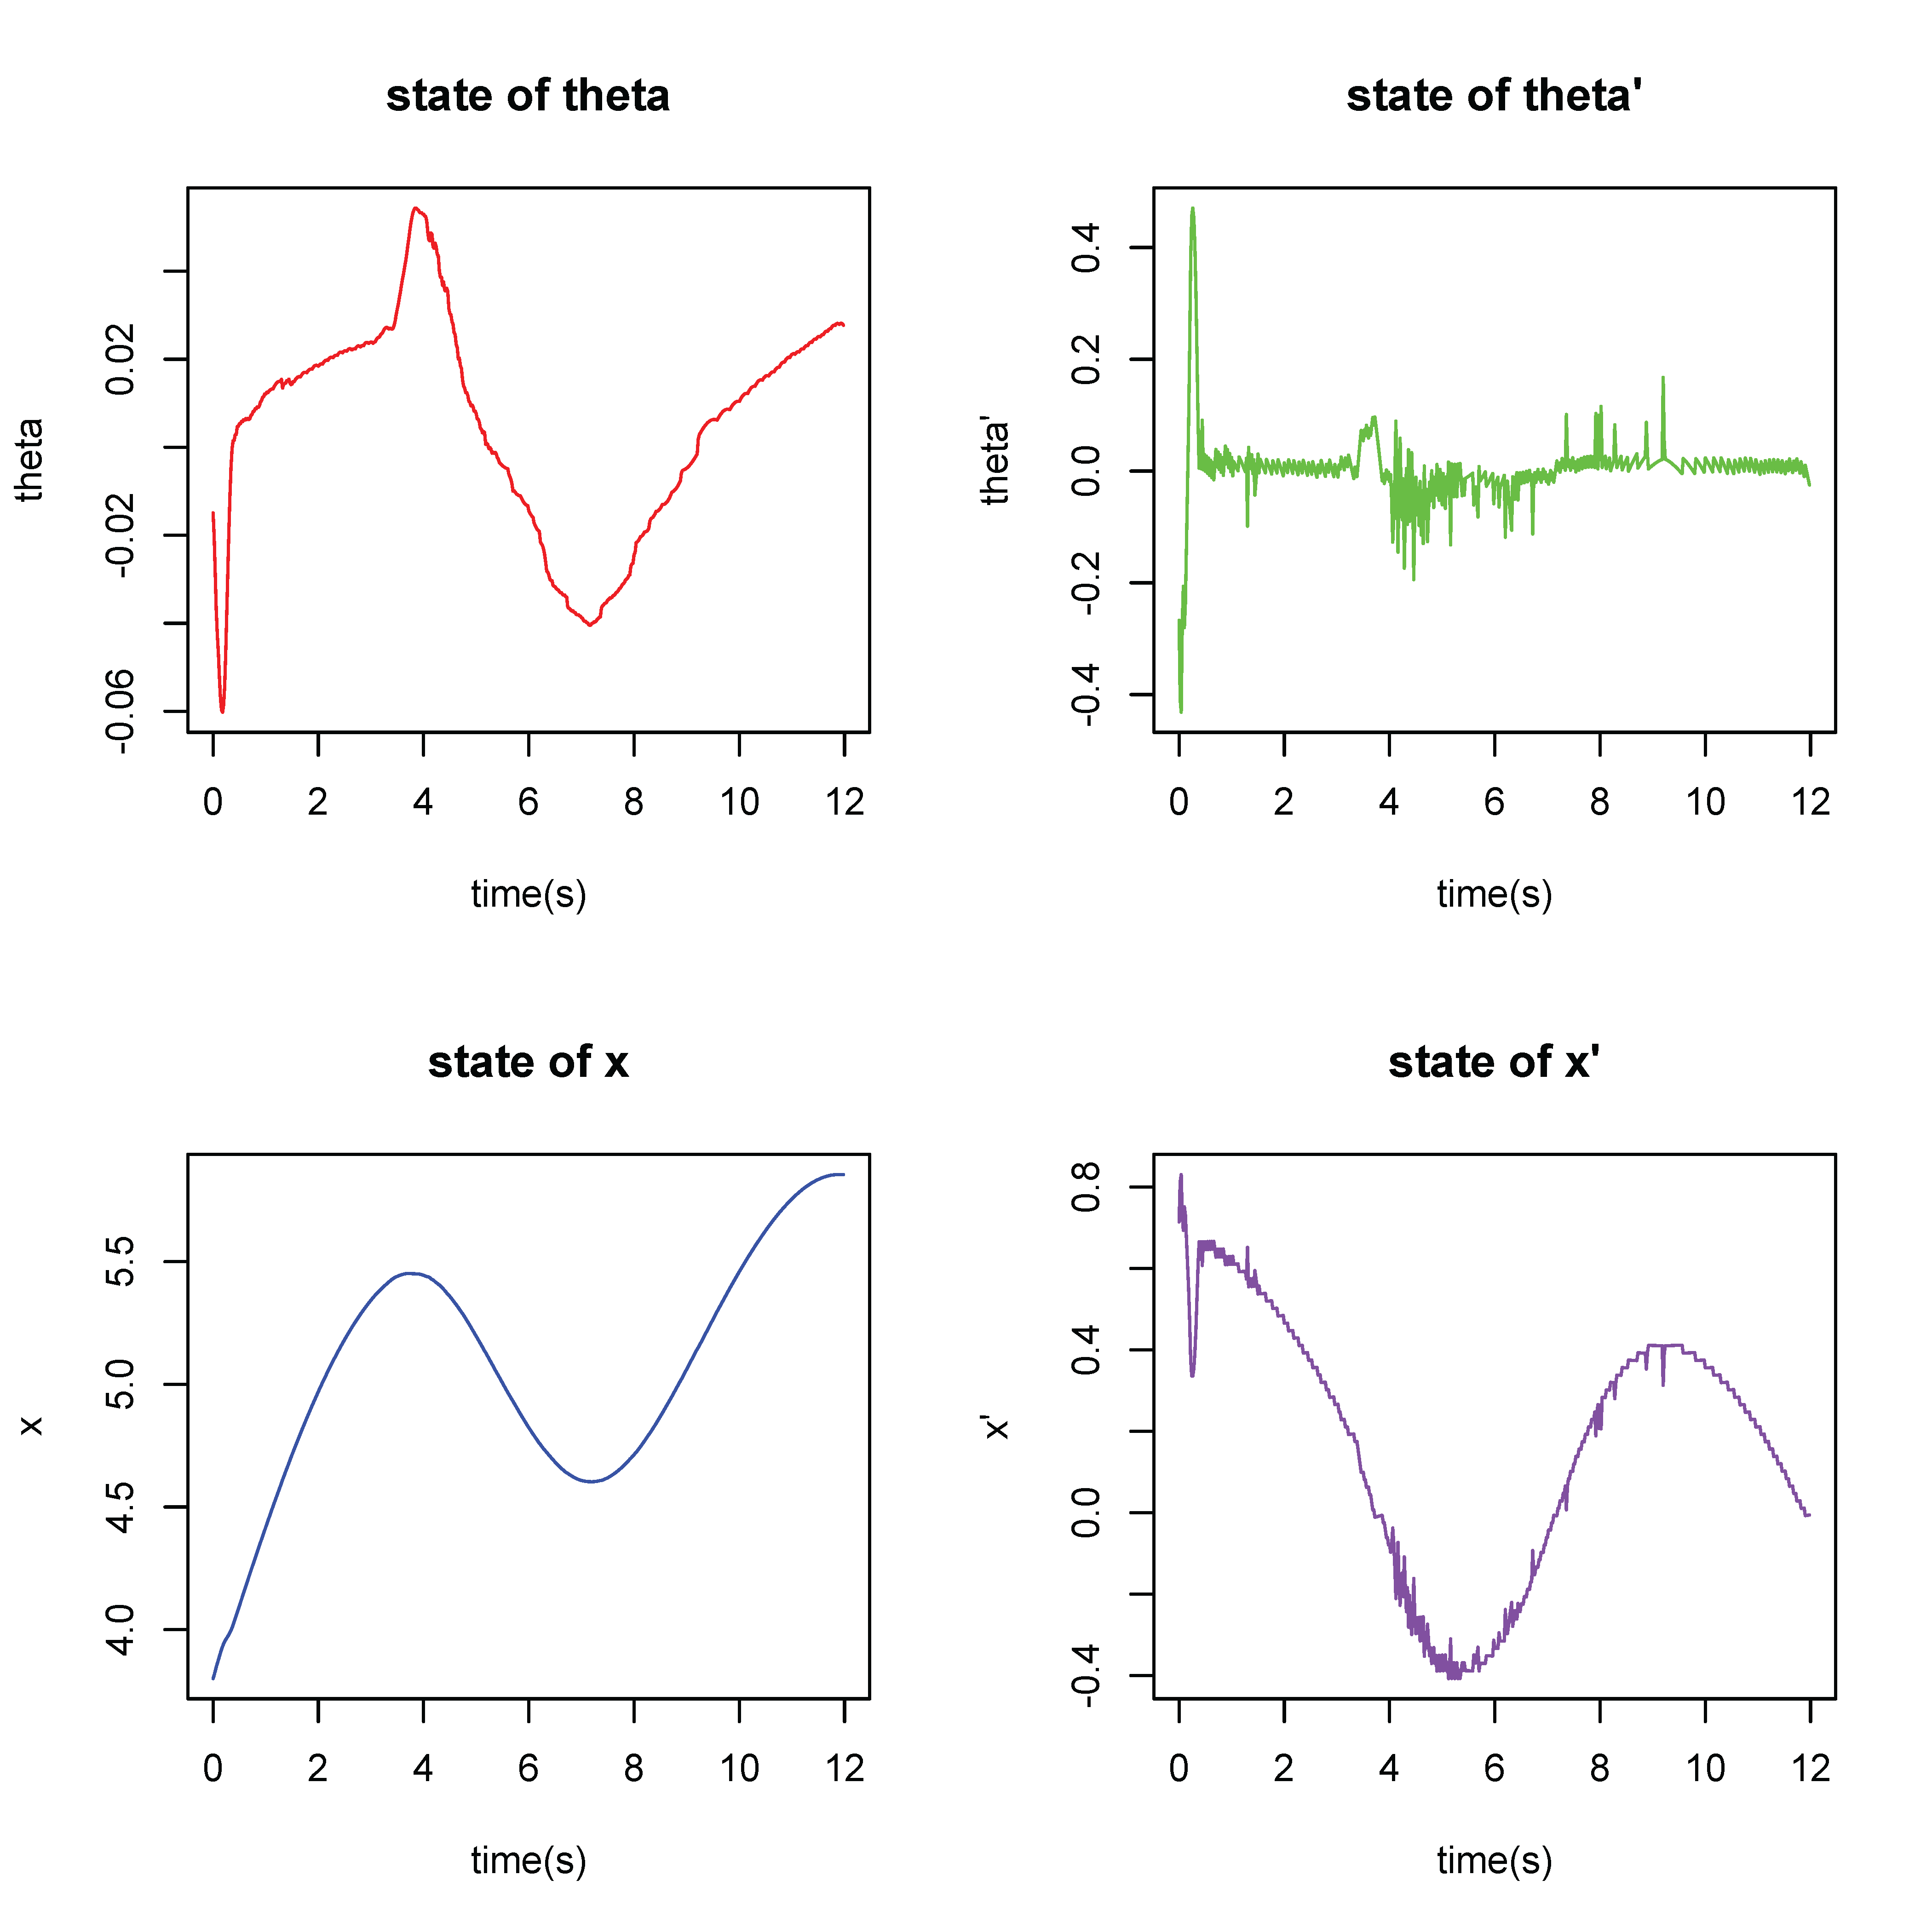
\includegraphics[width=14cm]{control-result.png}
\caption{Control Result of the control model based on Gaussian
  process. In the model, forces from -5 to 5 (only integers) could be
  used. The system is simulated using the physical model.}
\label{control-result}
\end{figure}

The control model we devised shows a successful control. In figure
\ref{control-error}, we can find that the prediction error drops
rapidly when the model continues to control the system. After 4s, the
system nearly don't need to learn from the observations. 

\begin{figure}[!]
\centering
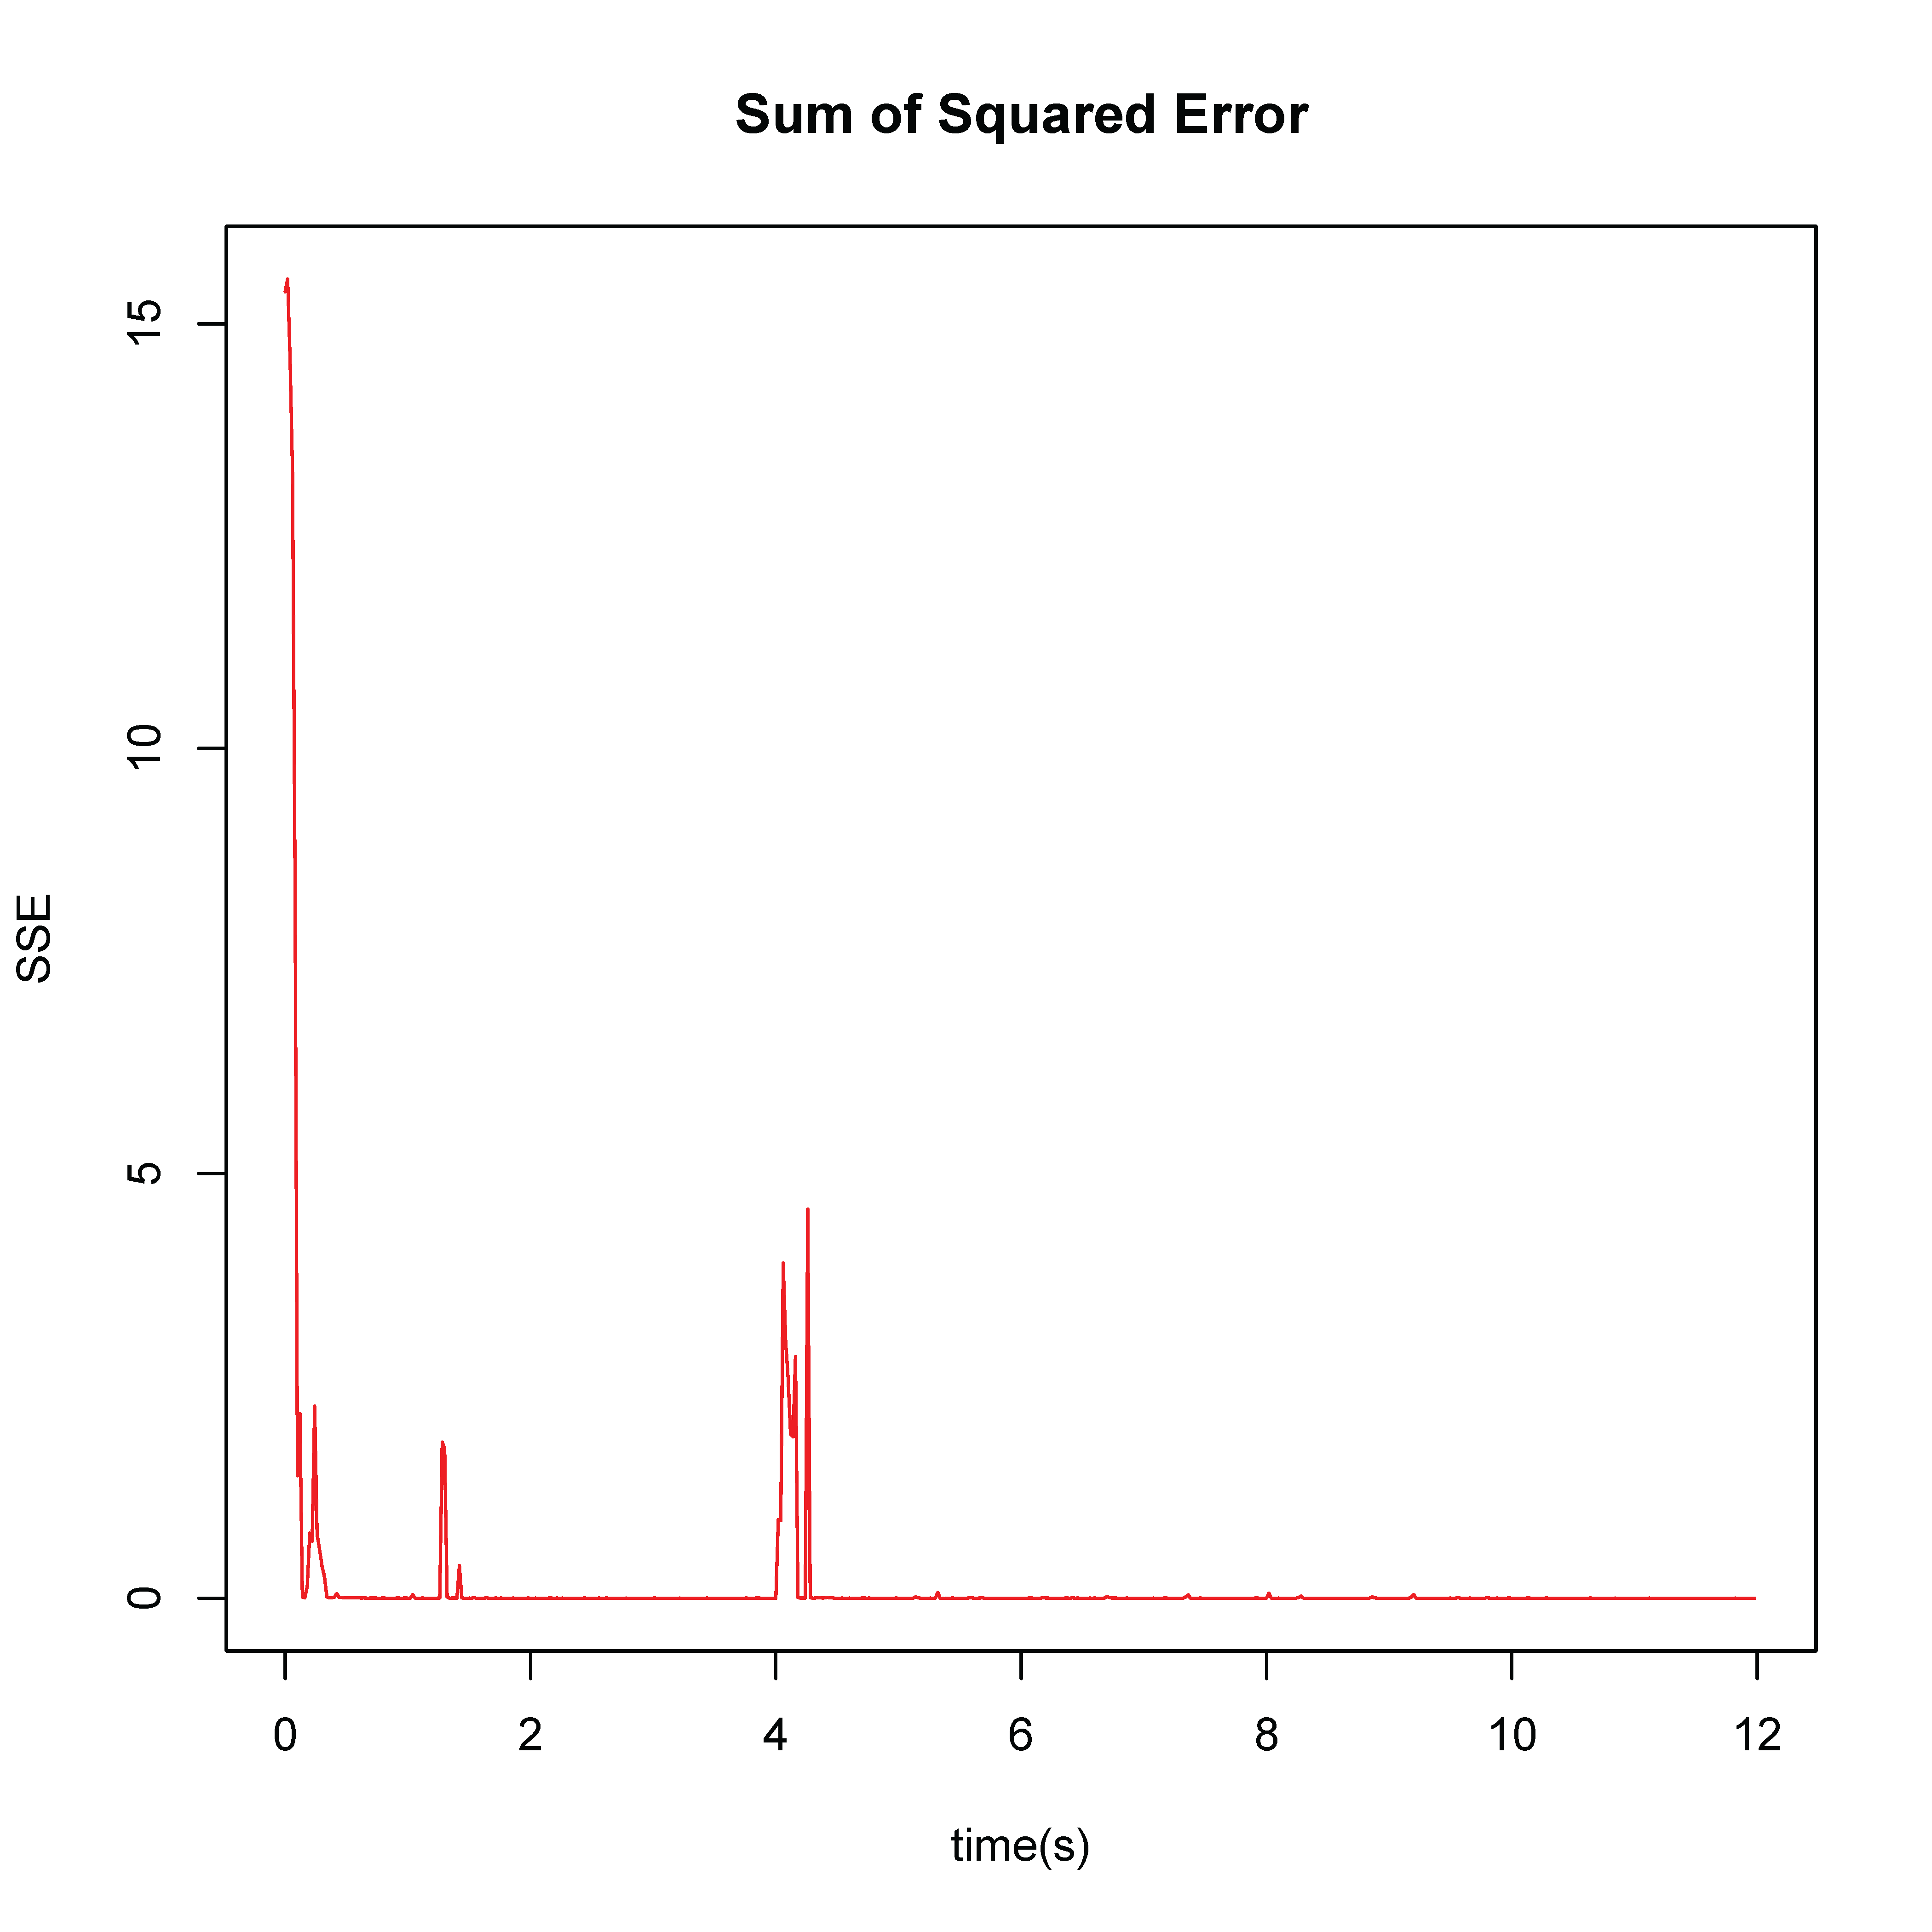
\includegraphics[width=8cm]{control-error.png}
\caption{Sum of Squared Error(SSE) between the prediction and the real
  observation during the control process. As we can see from 4s, the
  SSE drops to zero and nearly no addtional data should be learned.}
\label{control-error}
\end{figure}

In the control model, the prediction seems to be more accurate than in
the learning model. The reason why this happens is that, after the
system run for a certain period, its state lies in a relatively small
vector space and stabelizes (hardly goes out of this range). So
there are much training data in this range, which helps the Gaussian
process to predict more accurately.\\

\section{Conclusion}

In this project, we start from the study of a physical system
(cart-pole). Then we go through the Gaussian process regression. And
based on the simulation core of the cart-pole system and prediction of
the Gaussian process, we devised a learning model to predict the
behavior of cart-pole system and a control model to make
control-signal decision.

In the result analysis, we find that these two models work really
well. And we can also conclude that the training data is very
essential to the Gaussian process. Not only the size of the training
data, but also the distribution affects the regression result of
Gaussian process a lot.

\section{Acknowledgement}
This project is from the course ''Projects in Artificial Intelligence and Machine Learning'' WS 2013/14, which are supported by TUB-Lab KI and Professor Dr. Manfred Opper. Special thanks to our supervisors Florian Stimberg and Andreas Ruttor for the supports and helps in this project.

\newpage
\bibliographystyle{plain}
\bibliography{Report}{}
\end{document}
